%%%%%%%%%%%%%%%%%%%%%%%%%%%%%%%%%%%%%%%%%%%%%%%%%%%%%%%%%%%%%%%%%%%%%%%%%%%%%%%%%%%%%%%%%%%%%%%
%% Description:       Programmentwurf advanced software engineering
%% Author:      Manuel Berg, m.berg@enbw.com
%%  -*- coding: utf-8 -*-
%%%%%%%%%%%%%%%%%%%%%%%%%%%%%%%%%%%%%%%%%%%%%%%%%%%%%%%%%%%%%%%%%%%%%%%%%%%%%%%%%%%%%%%%%%%%%%%

\documentclass[
   ngerman          % neue deutsche Rechtschreibung
  ,a4paper          % Papiergrösse
% ,twoside          % Zweiseitiger Druck (rechts/links)
% ,10pt             % Schriftgrösse
%  ,11pt
  ,12pt
  ,pdftex
%  ,disable         % Todo-Markierungen auschalten
]{report}

% Codierung der Dateien auswählen:
% \usepackage[latin1]{inputenc}    % Für UNIX mit ISO-LATIN-codierten Dateien
% \usepackage[applemac]{inputenc}  % Für Apple MacOS
% \usepackage[ansinew]{inputenc}   % Für Microsoft Windows
\usepackage[utf8]{inputenc}        % UTF-8 codierte Dateien, Unix

\usepackage{bericht}
\usepackage[document]{ragged2e}
\usepackage{scrlayer-scrpage}
\usepackage{titlesec}
\usepackage{setspace}
\usepackage[backend=bibtex,style=numeric-comp,sorting=none]{biblatex}
\usepackage{makecell}
\usepackage{diagbox}
\setlength\bibitemsep{1.5\itemsep}
\addbibresource{bericht.bib}

%% ACHTUNG, wenn man eine eigene Formatdatei (bericht.fmt) benutzt, werden Änderungen an bericht.sty
%% erst wirksam, wenn die Format-Datei neu erzeugt wurde!
%% (Genauer: Alle Änderungen, die textuell vor der nächsten Zeile ".... endofdump...." stehen
%% werden erst wirksam, wenn die Formatdatei neu erzeugt wurde)
\csname endofdump\endcsname

%%%%%%%%%%%%%%%%%%%%%%%%%%%%%%%%%%%%%%%%%%%%%%%%%%%%%%%%%%%%%%%%%%%%%%%%%%%%%%%
%% Angaben zur Arbeit
%%%%%%%%%%%%%%%%%%%%%%%%%%%%%%%%%%%%%%%%%%%%%%%%%%%%%%%%%%%%%%%%%%%%%%%%%%%%%%%

\newcommand{\Autor}{Nadine Weiß und Manuel Berg}
\newcommand{\MatrikelNummer}{3196898, 5931590}
\newcommand{\Kursbezeichnung}{TINF19B5}

\newcommand{\FirmenName}{EnBW Energie Baden-Württemberg AG}
\newcommand{\FirmenStadt}{Durlacher Allee 93, 76131 Karlsruhe}
\newcommand{\FirmenLogoDeckblatt}{\includegraphics[width=6cm]{enbw}}

\newcommand{\BetreuerFirma}{Andreas Adler, Roman Walz}
%\newcommand{\BetreuerDHBW}{Titel Vorname Nachname}

%%%%%%%%%%%%%%%%%%%%%%%%%%%%%%%%%%%%%%%%%%%%%%%%%%%%%%%%%%%%%%%%%%%%%%%%%%%%%%%%%%%%%

% Wird auf dem Deckblatt und in der Erklärung benutzt:
\newcommand{\Was}{Programmentwurf}
%\newcommand{\Was}{Studienarbeit}
%\newcommand{\Was}{Bachleorarbeit}

%%%%%%%%%%%%%%%%%%%%%%%%%%%%%%%%%%%%%%%%%%%%%%%%%%%%%%%%%%%%%%%%%%%%%%%%%%%%%%%%%%%%%

\newcommand{\Titel}{\enquote{Mensch ärgere Dich nicht}}

\newcommand{\AbgabeDatum}{31.\,05.\,2022}

%\newcommand{\Dauer}{12 Wochen}

%\newcommand{\Abschluss}{Bachelor of Science}

\newcommand{\Studiengang}{Informatik}

\newcommand{\Studiengangsleiter}{Maurice Müller}

\newcommand{\uproman}[1]{\uppercase\expandafter{\romannumeral#1}}
% Befehl für grosse römische Zahlen

\newcommand{\abkspace}{\hspace{1.2cm}}

\newcommand{\myemph}[1]{\textbf{\texttt{#1}}}

\definecolor{light-gray}{gray}{0.85}
%\definecolor{eclipseBlue}{RGB}{42,0.0,255}
%\definecolor{eclipseGreen}{RGB}{63,127,95}
%\definecolor{eclipsePurple}{RGB}{127,0,85}

\hypersetup{%%
  pdfauthor={Manuel Berg},
  pdftitle={Vorlesungsprotokoll},
  pdfsubject={Theoretische Grundlagen der Kommunikation}
}

%\setcounter{secnumdepth}{3}

%%%%%%%%%%%%%%%%%%%%%%%%%%%%%%%%%%%%%%%%%%%%%%%%%%%%%%%%%%%%%%%%%%%%%%%%%%%%%%%

% Wenn \includeonly{..} benutzt wird, werden nur diese Kaptitel ausgegeben.
\includeonly{
  abk
 ,kapitel1
 ,kapitel2
 ,kapitel3
 ,kapitel4
 ,kapitel5
}

%%%%%%%%%%%%%%%%%%%%%%%%%%%%%%%%%%%%%%%%%%%%%%%%%%%%%%%%%%%%%%%%%%%%%%%%%%%%%%%

% Benutzt man das "biblatex"-Paket, dann muss das hier stehen:
% siehe auch die mit BIBLATEX markierten Zeilen in bericht.sty
%\addbibresource{bericht.bib}

\begin{document}

%%%%%%%%%%%%%%%%%%%%%%%%%%%%%%%%%%%%%%%%%%%%%%%%%%%%%%%%%%%%%%%%%%%%%%%%%%%%%%%

\begin{titlepage}
\begin{center}
\vspace*{-2cm}
\hfill
\includegraphics[width=4.5cm]{dhbw-logo}\\[2cm]
{\Huge \Titel}\\[1.5cm]
{\Huge\scshape \Was}\\[1.5cm]
{\large in der Vorlesung \glqq Advanced Software Engineering\grqq}\\[0.5cm]
{\large im fünften und sechsten Semester}\\[0.5cm]
{\large des Studienganges \Studiengang}\\[0.5cm]
{\large an der}\\[0.5cm]
{\large Dualen Hochschule Baden-Württemberg Karlsruhe}\\[0.5cm]
{\large von}\\[0.5cm]
{\large\bfseries \Autor}\\[1cm]
{\large \AbgabeDatum}
\vfill
\end{center}
\begin{tabular}{l@{\hspace{2cm}}l}
%Bearbeitungszeitraum	         & \Dauer 			\\
Matrikelnummern	                 & \MatrikelNummer		\\
Kurs			         & \Kursbezeichnung		\\
%Ausbildungsbetrieb	         & \FirmenName			\\
			         %& \FirmenStadt			\\
%Betreuer des Ausbildungsbetriebes	 & \BetreuerFirma		\\
%Gutachter der dualen Hochschule	 & \BetreuerDHBW		\\
Dozent	 & \Studiengangsleiter		\\
\end{tabular}
\end{titlepage}

%%%%%%%%%%%%%%%%%%%%%%%%%%%%%%%%%%%%%%%%%%%%%%%%%%%%%%%%%%%%%%%%%%%%%%%%%%%%%%%

%%%%%%%%%%%%%%%%%%%%%%%%%%%%%%%%%%%%%%%%%%%%%%%%%%%%%%%%%%%%%%%%%%%%%%%%%%%%%%%%%%%%%%%%%%%%%%%
%% Description:       Programmentwurf advanced software engineering
%% Author:      Manuel Berg, m.berg@enbw.com
%%  -*- coding: utf-8 -*-
%%%%%%%%%%%%%%%%%%%%%%%%%%%%%%%%%%%%%%%%%%%%%%%%%%%%%%%%%%%%%%%%%%%%%%%%%%%%%%%%%%%%%%%%%%%%%%%

\newpage
\
\onehalfspacing
\pagestyle{scrheadings}
\clearscrheadfoot
\pagenumbering{Roman}
\setcounter{page}{2}
\ofoot[\pagemark]{\pagemark}
%\thispagestyle{empty}
\vspace{-0.7cm}
\justify 
\begin{framed}
\begin{center}
\Large\bfseries Eidesstattliche Erklärung
\end{center}
%\medskip
\noindent
\begin{center}
(gemäß §5(3) der \enquote{Studien- und Prüfungsordnung DHBW Technik} vom 29.\,09.\,2017)\\
\end{center}
Ich versichere hiermit, dass ich mein \Was\ vom 31.\,05.\,2022 mit dem Thema
\enquote{Mensch ärgere Dich nicht}
selbstständig verfasst und keine anderen als die angegebenen Quellen und Hilfsmittel benutzt habe.
\vspace{0.5cm}
%\noindent
%\underline{\hspace{4cm}}\hfill\underline{\hspace{6cm}}\\
%Ort~~~~~Datum\hfill Unterschrift\hspace{4cm}

%% Ort und Datum  
%%\vspace{1,5 cm} 
%\begin{tabular}{p{7cm}p{.5cm}l}
%\dotfill \\ 
%Ort, Datum
%\end{tabular}% 
%
%% Hier kommen die Unterschriten hin
%%\vspace{1,5 cm} 
%\begin{tabular}{p{7cm}p{.5cm}l}
%\dotfill \\ 
%Unterschrift 
%\end{tabular}%
\begin{center}
\hspace*{\fill}\begin{tabular}{@{}l@{}}\hline
\makebox[15.3cm]{Ort, Datum \hspace{7cm} Unterschrift}
\end{tabular}
\end{center}




\end{framed}

\newpage
\onehalfspacing

%\vspace{-3cm}
%\begin{framed}
%\begin{center}
%\Large\bfseries Sperrvermerk
%\end{center}
%\medskip
%\noindent
%Die  vorliegende  Projektarbeit  beinhaltet  interne  und  vertrauliche  Informationen  der EnBW  Energie Baden-Württemberg  AG, der  EnBW  Kernkraft  GmbH, sowie der Gesellschaft für nukleares Reststoffrecycling mbH.  Die Weitergabe des Inhalts dieser Arbeit, beiliegender Zeichnungen oder anderer Daten im  Gesamten  oder  in  Teilen  ist  grundsätzlich  untersagt.  Es  dürfen  keinerlei  Kopien oder Abschriften -- in schriftlicher oder digitaler Form -- angefertigt oder verteilt werden. Ausnahmen  bedürfen  der  schriftlichen  Genehmigung  der beteiligten Unternehmen.  Die  Arbeit  ist  nur  den  Korrektoren  sowie  den  Mitgliedern  des Prüfungsausschusses zugänglich zu machen.
%\end{framed}

\vspace{9cm}
\newcommand{\latex}{\LaTeX\xspace}
\begin{framed}
\justify \textbf{Hinweis:} Der \latex-Quellcode dieses Dokumentes basiert auf der \href{https://www.karlsruhe.dhbw.de/inf/studienverlauf-organisatorisches.html}{\enquote{Vorlage für Berichte der DHBW Karlsruhe}}, welche freundlicherweise von \href{mailto:juergen.vollmer@dhbw-karlsruhe.de}{Prof.\,Dr.\:Jürgen Vollmer} zur Verfügung gestellt wurde.
%\end{flushleft}
\end{framed}


%%%%%%%%%%%%%%%%%%%%%%%%%%%%%%%%%%%%%%%%%%%%%%%%%%%%%%%%%%%%%%%%%%%%%%%%%%%%%%%
\endinput
%%%%%%%%%%%%%%%%%%%%%%%%%%%%%%%%%%%%%%%%%%%%%%%%%%%%%%%%%%%%%%%%%%%%%%%%%%%%%%%


%%%%%%%%%%%%%%%%%%%%%%%%%%%%%%%%%%%%%%%%%%%%%%%%%%%%%%%%%%%%%%%%%%%%%%%%%%%%%%%
%\justify
%\vspace*{-6cm}
%\begin{abstract}
%\thispagestyle{plain}
%\setcounter{page}{4}
%Das Thema der Projektarbeit ist die Einführung eines Intranets mit Anbindung an Informationsbildschirme innerhalb der kritischen Infrastruktur der Gesellschaft für nukleares Reststoffrecycling mbH (\acs{GNR}). Um dies zu ermöglichen, ist zunächst eine genaue Analyse der Rahmenbedingungen notwendig. Das grobe Lastenheft, welches zum Beginn der Projektarbeit vorliegt, muss in Absprache mit der Geschäftsführung der \acs{GNR} unter Berücksichtigung technischer Möglichkeiten verfeinert werden. Im Rahmen eines ausführ\-lichen Produktvergleiches sollen die am Markt verfügbaren Optionen aufgezeigt werden, unter denen abgewogen werden muss. Ein zentraler Aspekt der gesamten Projektarbeit ist, dass das Intranet eine einfache und übersichtliche Möglichkeit zur redaktionellen Pflege der Inhalte bieten soll. Falls sich bei dem gewählten Produkt mehrere mögliche Implementierungsvarianten anbieten, so soll eine Empfehlung unter Berücksichtigung des besonderen Anwendungsfalls bei der \acs{GNR} ausgesprochen werden. Für die Informationsbildschirme an den Standorten der \acs{GNR} ist gemäß dem Lastenheft eine gesonderte Intranet-Seite aufzubauen. Das gesamte Projekt ist weitestmöglich in den Produktivbetrieb zu überführen, sofern es die informationstechnischen Sicherheitsprüfungen und der eventuelle Einsatz von Fremdpersonal zeitlich zulassen.\\
%
%\vspace{0.5cm}
%\begin{center}
%\textbf{Abstract}
%\end{center}
%The topic of this project is the introduction of an intranet with connection to information monitors within the critical infrastrucure given at \acs{GNR}. In order to achieve this, it is necessary to thoroughly analyse the general conditions of the present environment. The vague requirement specification which exists upon the start of this project has to be refined in consultation with the executive board of \acs{GNR}, keeping the technical possibilities in mind. An extensive comparison of the available products will be conducted. One key aspect of the whole project is that the intranet should offer an easy and comprehensible way to allow editorial maintenance. Should the chosen product offer multiple variants of implementation, a decision should be made considering the special use case at \acs{GNR}. According to the requirement specification, a separate intranet page for the information monitors will be built. The whole project is to be implemented as far as the IT security guidelines and the possible hiring of external staff allow it.
%
%\end{abstract}

\newpage
\pagestyle{scrheadings}
\clearscrheadfoot
\pagenumbering{Roman}
\setcounter{page}{4}
\ofoot[\pagemark]{\pagemark}
\pdfbookmark[section]{\contentsname}{toc}
\tableofcontents           % Inhaltsverzeichnis hier ausgeben
\listoffigures             % Liste der Abbildungen
\addcontentsline{toc}{chapter}{\listfigurename}
\listoftables              % Liste der Tabellen
\addcontentsline{toc}{chapter}{\listtablename}
%\lstlistoflistings         % Liste der Listings
%\listofequations           % Liste der Formeln

% Jetzt kommt der "eigentliche" Text
%%%%%%%%%%%%%%%%%%%%%%%%%%%%%%%%%%%%%%%%%%%%%%%%%%%%%%%%%%%%%%%%%%%%%%%%%%%%%%%
%% Descr:       Sitzungsprotokoll Psych. Grundlagen für Informatiker
%% Author:      Manuel Berg, m.berg@enbw.com
%%  -*- coding: utf-8 -*-
%%%%%%%%%%%%%%%%%%%%%%%%%%%%%%%%%%%%%%%%%%%%%%%%%%%%%%%%%%%%%%%%%%%%%%%%%%%%%%%

\chapter*{Abkürzungsverzeichnis}                   % chapter*{..} -->   keine Nummer, kein "Kapitel"
						         				   % Nicht ins Inhaltsverzeichnis
						         				   
\addcontentsline{toc}{chapter}{Akürzungsverzeichnis}   % Damit das doch ins Inhaltsverzeichnis kommt

% Hier werden die Abkürzungen definiert
\begin{acronym}[DHBW]

% \acro{Name}{Darstellung der Abkürzung}{Langform der Abkürzung}

\acro{BSI}[BSI]{\abkspace Bundesamt für Sicherheit in der Informationstechnik}
\acro{GI}[GI]{\abkspace Gesellschaft für Informatik e.V.}

 % Wenn nicht benutzt, erscheint diese Abk. nicht in der Liste
 %\acro{NUA}{Not Used Acronym}
 
\end{acronym}
              % Abkürzungsverzeichnis
%%%%%%%%%%%%%%%%%%%%%%%%%%%%%%%%%%%%%%%%%%%%%%%%%%%%%%%%%%%%%%%%%%%%%%%%%%%%%%%%%%%%%%%%%%%%%%%
%% Description:       Programmentwurf advanced software engineering
%% Author:      Manuel Berg, m.berg@enbw.com
%%  -*- coding: utf-8 -*-
%%%%%%%%%%%%%%%%%%%%%%%%%%%%%%%%%%%%%%%%%%%%%%%%%%%%%%%%%%%%%%%%%%%%%%%%%%%%%%%%%%%%%%%%%%%%%%%

\titlespacing*{\chapter}{0pt}{-30mm}{10pt}
\titleformat{\chapter}[display]
  {\normalfont\bfseries}{}{10pt}{\Huge\thechapter.\quad}
  
\chapter{Einführung (4P)}
\pagestyle{scrheadings}
\clearscrheadfoot
\pagenumbering{arabic}
\setcounter{page}{1}
\ofoot[\pagemark]{\pagemark}
%\ohead[\headmark]{\headmark}
\onehalfspacing

\section{Übersicht über die Applikation (1P)}
\emph{[Was macht die Applikation? Wie funktioniert sie? Welches Problem löst sie/welchen Zweck hat sie?]}
\\
\\
\noindent Die Applikation dient rein der Unterhaltung und simuliert das bekannte deutsche Gesell\-schaftsspiel \emph{Mensch ärgere Dich nicht} mit dem klassischen Spielfeld für vier Spieler. Hierbei kann -- entsprechend dem originalen Brettspiel -- zwischen zwei, drei oder vier Teilnehmenden gewählt werden. Eine Besonderheit der Applikation besteht darin, dass nicht alle Teilnehmenden \enquote{menschlich} sein müssen, sondern nach Belieben auch ein Algorithmus das Würfeln und die Ausführung der Züge übernehmen kann. ToDo: Funktionsweise; Glossar mit Erklärung Spielbrett, Spielfeld

\section{Wie startet man die Applikation? (1P)}
\emph{[Wie startet man die Applikation? Was für Voraussetzungen werden benötigt? Schritt-für-Schritt-Anleitung]}
\\
\\
\noindent ToDo: Start in virtueller Ubuntu-Maschine ausprobieren

\section{Technischer Überblick (2P)}
\emph{[Nennung und Erläuterung der Technologien (z.B. Java, MySQL, ...), jeweils Begründung für den
Einsatz der Technologien]}
\\
\\
\noindent Als Programmiersprache wurde \textbf{\emph{Java}} verwendet, da dies in den Anforderungen bereits definiert wurde und wir mit dieser Sprache bisher die meisten Erfahrungen gesammelt haben. Auch in der Vorlesung \enquote{Programmieren} im ersten und zweiten Semester des Studienganges wurden die Grundlagen objektorientierter Programmiersprachen anhand von Java erläutert, weshalb sich dies auch für den Programmentwurf angeboten hat. Bezüglich der \acs{GUI} ist die Entscheidung auf das Framework \textbf{\emph{Swing}} gefallen. Auch hier haben wir in der genannten Vorlesung und auch privat bereits Erfahrungen sammeln können. Da der Fokus des Programmentwurfs nicht auf der \acs{GUI} liegen sollte, haben wir hier die für uns einfachste Variante ausgewählt. Die selben Argumente haben uns auch zu der Entscheidung für das Abhängigkeitsmanagement mit \textbf{\emph{Maven}} geführt.
%%%%%%%%%%%%%%%%%%%%%%%%%%%%%%%%%%%%%%%%%%%%%%%%%%%%%%%%%%%%%%%%%%%%%%%%%%%%%%%%%%%%%%%%%%%%%%%
%% Description:       Programmentwurf advanced software engineering
%% Author:      Manuel Berg, m.berg@enbw.com
%%  -*- coding: utf-8 -*-
%%%%%%%%%%%%%%%%%%%%%%%%%%%%%%%%%%%%%%%%%%%%%%%%%%%%%%%%%%%%%%%%%%%%%%%%%%%%%%%%%%%%%%%%%%%%%%%

\titlespacing*{\chapter}{0pt}{-30mm}{10pt}
\titleformat{\chapter}[display]
  {\normalfont\bfseries}{}{10pt}{\Huge\thechapter.\quad}
  
\chapter{Clean Architecture (8P)}
\pagestyle{scrheadings}
\clearscrheadfoot
\pagenumbering{arabic}
\setcounter{page}{2}
\ofoot[\pagemark]{\pagemark}
%\ohead[\headmark]{\headmark}
\onehalfspacing

\section{Was ist Clean Architecture? (1P)}
\emph{[Allgemeine Beschreibung der Clean Architecture in eigenen Worten]}

\section{Analyse der Dependency Rule (2P)}
\emph{[1 Klasse, die die Dependency Rule einhält und 1 Klasse, die die Dependency Rule verletzt; jeweils
UML der Klasse und Analyse der Abhängigkeiten in beide Richtungen (d.h., von wem hängt die Klasse
ab und wer hängt von der Klasse ab) in Bezug auf die Dependency Rule]}

\subsubsection{Positiv-Beispiel: Dependency Rule}
\subsubsection{Negativ-Beispiel: Dependency Rule}

\section{Analyse der Schichten (5P)}
\emph{[jeweils 1 Klasse zu 2 unterschiedlichen Schichten der Clean-Architecture: jeweils UML der Klasse
(ggf. auch zusammenspielenden Klassen), Beschreibung der Aufgabe, Einordnung mit Begründung in
die Clean-Architecture]}

\subsubsection{Schicht: [Name]}
\subsubsection{Schicht: [Name]}
%%%%%%%%%%%%%%%%%%%%%%%%%%%%%%%%%%%%%%%%%%%%%%%%%%%%%%%%%%%%%%%%%%%%%%%%%%%%%%%%%%%%%%%%%%%%%%%
%% Description:       Programmentwurf advanced software engineering
%% Author:      Manuel Berg, m.berg@enbw.com
%%  -*- coding: utf-8 -*-
%%%%%%%%%%%%%%%%%%%%%%%%%%%%%%%%%%%%%%%%%%%%%%%%%%%%%%%%%%%%%%%%%%%%%%%%%%%%%%%%%%%%%%%%%%%%%%%

\titlespacing*{\chapter}{0pt}{-30mm}{10pt}
\titleformat{\chapter}[display]
  {\normalfont\bfseries}{}{10pt}{\Huge\thechapter.\quad}
  
\chapter{SOLID (8P)}
\pagestyle{scrheadings}
\clearscrheadfoot
\pagenumbering{arabic}
\setcounter{page}{3}
\ofoot[\pagemark]{\pagemark}
%\ohead[\headmark]{\headmark}
\onehalfspacing

\section{Analyse SRP (3P)}
\emph{[Jeweils eine Klasse als positives und negatives Beispiel für SRP; jeweils UML der Klasse und
Beschreibung der Aufgabe bzw. der Aufgaben und möglicher Lösungsweg des Negativ-Beispiels (inkl.
UML)]}

\subsubsection{Positiv-Beispiel}
\begin{figure}[htbp]
\centering
\centerline{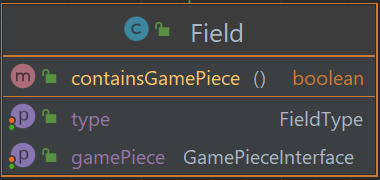
\includegraphics[scale=.6]{positivbeispiel_srp}}
\caption{Positiv-Beispiel SRP [Eigene Darstellung aus \emph{IntelliJ}]}
\label{fig:positivbeispiel_srp}
\end{figure}
\noindent Die Klasse \emph{Field} stellt als einzige Aufgabe ein Spielfeld dar. Dieses kann einem Typen zugeordnet sein, und optional eine Spielfigur enthalten. Durch einen Methodenaufruf wird zurückgegeben, ob sich eine Spielfigur auf dem entsprechenden Feld befindet. Das Single Responsibility Principle wird durch die hier dargestellte Klasse nicht verletzt.

\subsubsection{Negativ-Beispiel}
\begin{figure}[htbp]
\centering
\centerline{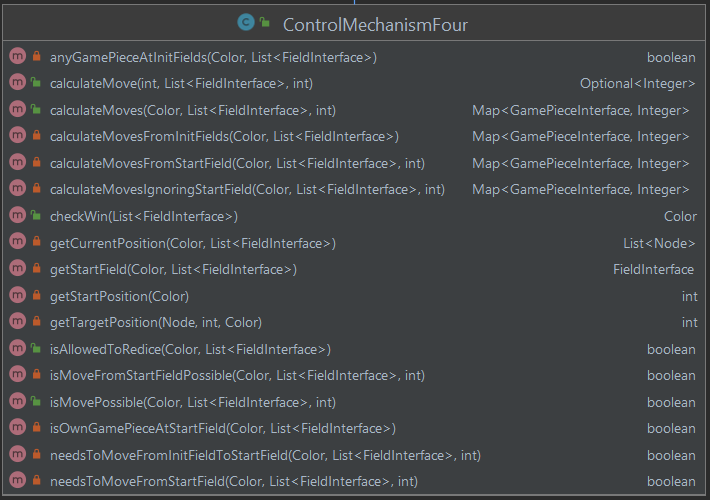
\includegraphics[scale=.6]{negativbeispiel_srp}}
\caption{Negativ-Beispiel SRP [Eigene Darstellung aus \emph{IntelliJ}]}
\label{fig:negativbeispiel_srp}
\end{figure}
\newpage
\noindent Die Klasse \emph{ControlMechanismFour} ist dafür verantwortlich, 
\begin{itemize}
\item mögliche Züge zu berechnen,
\item zu prüfen, ob ein Spieler bereits gewonnen hat,
\item zu prüfen, ob ein Spieler nochmals würfeln darf und
\item zu prüfen, ob ein Spieler überhaupt einen Zug durchführen kann.
\end{itemize}


\noindent Es wird deutlich, dass die Klasse für mehrere Tätigkeiten verantworlich ist und somit das Single Responsibility Principle verletzt wird. Um das Prinzip einhalten zu können, sollte der Umfang der Klasse auf die Erfüllung einer einzigen Aufgabe reduziert werden. Hierzu könnte \emph{ControlMechanismFour} in zwei neue Klassen aufgeteilt werden. Dabei wäre eine Klasse für die Berechnung der Züge verantworlich; die andere prüft das weitere mögliche Vorgehen eines Spielers. 

Außerdem enthält \emph{ControlMechanismFour} sieben private Methoden, welche in eine Hilfsklasse ausgelagert werden sollten. Diese privaten Methoden sind in \hyperref[fig:negativbeispiel_srp]{Abbildung 3.2} mit roten Schloss-Symbolen gekennzeichnet. Eine Auslagerung ist sinnvoll, weil die Methoden nicht nur in \emph{ControlMechanismFour} Verwendung finden, sondern auch in anderen Klassen (wie beispielsweise in der \emph{Graph}-Klasse) aufgerufen werden. Hierdurch wird redundanter Quellcode eingespart.

\newpage
\noindent

\section{Analyse OCP (3P)}
\emph{[Jeweils eine Klasse als positives und negatives Beispiel für OCP; jeweils UML der Klasse und
Analyse mit Begründung, warum das OCP erfüllt/nicht erfüllt wurde – falls erfüllt: warum hier
sinnvoll/welches Problem gab es? Falls nicht erfüllt: wie könnte man es lösen (inkl. UML)?]}
\subsubsection{Positiv-Beispiel}
\begin{figure}[htbp]
\centering
\centerline{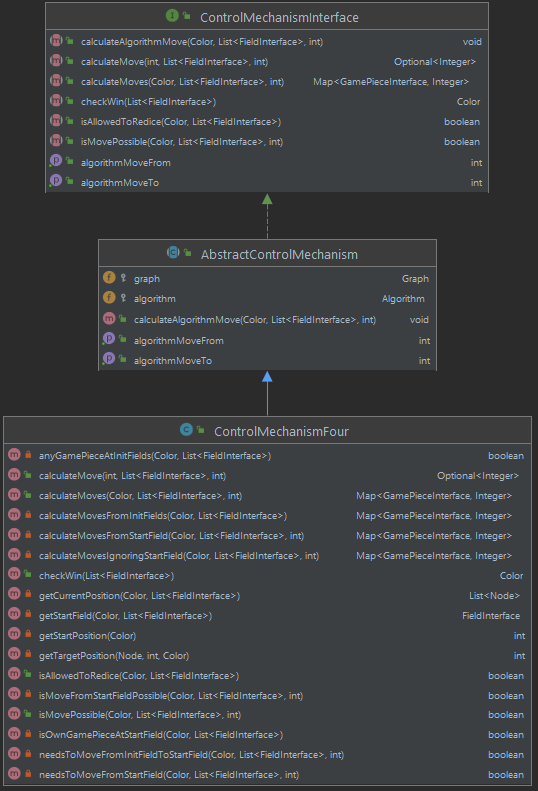
\includegraphics[scale=.5]{positivbeispiel_ocp}}
\caption{Positiv-Beispiel OCP [Eigene Darstellung aus \emph{IntelliJ}]}
\label{fig:positivbeispiel_ocp}
\end{figure}
\noindent Der \emph{ControlMechanism} ist offen für Erweiterungen bezüglich der Spieleranzahl. Dies wurde so entwickelt, da eine Abweichung von der Spielerzahl vier (z.B. Erhöhung auf sechs Spieler) eine optionale Anforderung des Projektes ist.
\newpage
\noindent Um beispielsweise einen \emph{ControlMechanism} für sechs Spieler umzusetzen, muss analog zur Klasse \emph{ControlMechanismFour} eine Klasse \emph{ControlMechanismSix} implementiert werden. Diese würde dann auch von \emph{AbstractControlMechanism} erben. 

Die Methoden werden immer über das \emph{ControlMechanismInterface} aufgerufen. Das bedeutet, ohne Änderungen an diesem kann das Verhalten wie oben dargestellt erweitert werden. Die OCP-Regel der verschlossenen Module gegenüber Modifikationen ist hierdurch erfüllt.

\subsubsection{Negativ-Beispiel}
\begin{figure}[htbp]
\centering
\centerline{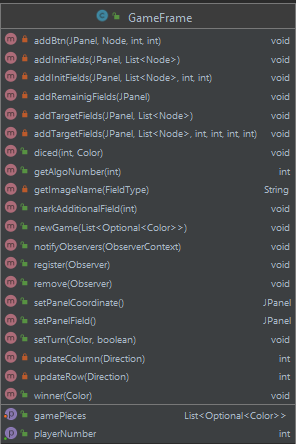
\includegraphics[scale=.6]{negativbeispiel_ocp}}
\caption{Negativ-Beispiel OCP [Eigene Darstellung aus \emph{IntelliJ}]}
\label{fig:negativbeispiel_ocp}
\end{figure}
\noindent ToDo: Negativ-Beispiel, weil wir hier nicht auf andere Spieleranzahlen erweitern können (Grafik)

\newpage
\section{Analyse LSP/ISP/DIP (2P)}
\emph{[Jeweils eine Klasse als positives und negatives Beispiel für entweder LSP oder ISP oder DIP); jeweils
UML der Klasse und Begründung, warum hier das Prinzip erfüllt/nicht erfüllt wird. Anm.: es darf nur ein Prinzip ausgewählt werden; es darf NICHT z.B. ein positives Beispiel für LSP und ein negatives Beispiel für ISP genommen werden]}

\subsubsection{Positiv-Beispiel DIP}
\begin{figure}[htbp]
\centering
\centerline{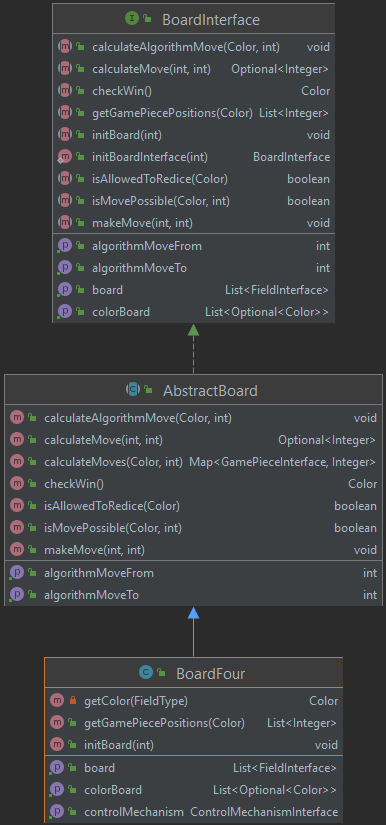
\includegraphics[scale=.45]{positivbeispiel_dip}}
\caption{Positiv-Beispiel DIP [Eigene Darstellung aus \emph{IntelliJ}]}
\label{fig:positivbeispiel_dip}
\end{figure}
\noindent Durch die Abstraktion des Spielbretts wird das Dependency Inversion Principle erfüllt, denn hier hängen die Details von Abstraktionen ab. In \hyperref[fig:positivbeispiel_dip]{Abbildung 3.5} ist zu erkennen, dass die Details -- also die konkreten Implementierungen -- in der Klasse \emph{BoardFour} zu finden sind.

\newpage 
\noindent Der Methodenaufruf beim Spielbrett ändert sich demnach nicht, wenn die konkrete Implementierung verändert wird. Beispielsweise könnte auch ein weiteres Spielbrett umgesetzt werden, ohne dass sich am restlichen Programm etwas ändert.

\subsubsection{Negativ-Beispiel DIP}
\begin{figure}[htbp]
\centering
\centerline{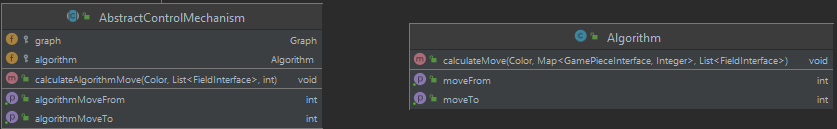
\includegraphics[scale=.6]{negativbeispiel_dip}}
\caption{Negativ-Beispiel DIP [Eigene Darstellung aus \emph{IntelliJ}]}
\label{fig:negativbeispiel_dip}
\end{figure}
\noindent Der \emph{ControlMechanism} steht in direkter Abhängigkeit der Klasse \emph{Algorithm}. Falls sich die Implementierung letzterer ändert, so muss auch \emph{AbstractControlMechanism} entsprechend angepasst werden. In dieser Zusammenstellung kann nur der vorhandene Algorithmus angewandt werden. Um dies zu umgehen und weitere Algorithmen verwenden zu können, wäre ein Interface sinnvoll.
%%%%%%%%%%%%%%%%%%%%%%%%%%%%%%%%%%%%%%%%%%%%%%%%%%%%%%%%%%%%%%%%%%%%%%%%%%%%%%%%%%%%%%%%%%%%%%%
%% Description:       Programmentwurf advanced software engineering
%% Author:      Manuel Berg, m.berg@enbw.com
%%  -*- coding: utf-8 -*-
%%%%%%%%%%%%%%%%%%%%%%%%%%%%%%%%%%%%%%%%%%%%%%%%%%%%%%%%%%%%%%%%%%%%%%%%%%%%%%%%%%%%%%%%%%%%%%%

\titlespacing*{\chapter}{0pt}{-30mm}{10pt}
\titleformat{\chapter}[display]
  {\normalfont\bfseries}{}{10pt}{\Huge\thechapter.\quad}
  
\chapter{Weitere Prinzipien (8P)}
\pagestyle{scrheadings}
\clearscrheadfoot
\pagenumbering{arabic}
\setcounter{page}{4}
\ofoot[\pagemark]{\pagemark}
%\ohead[\headmark]{\headmark}
\onehalfspacing

\section{Analyse GRASP: Geringe Kopplung (4P)}
\emph{[jeweils eine bis jetzt noch nicht behandelte Klasse als positives und negatives Beispiel geringer
Kopplung; jeweils UML Diagramm mit zusammenspielenden Klassen, Aufgabenbeschreibung der
Klasse und Begründung warum hier eine geringe Kopplung vorliegt bzw. Beschreibung, wie die
Kopplung aufgelöst werden kann]}

\subsubsection{Positiv-Beispiel}
\noindent Eine geringe Kopplung wurde durch den Einsatz des Observer-Patterns zwischen der für die Visualisierung zuständigen \enquote{GameFrame}-Klasse und der für den Spielablauf zuständigen \enquote{GameService}- Klasse erreicht. Das heißt, wenn in der UI durch den Benutzer eine Aktion ausgeführt wird, wird die \enquote{GameService}-Klasse benachrichtigt. Bei der Benachrichtigung weiß das benachrichtigende Objekt nichts Näheres über das zu benachrichtigende Objekt. Anders ausgedrückt, das Observable kennt nur die Observer-Schnittstelle. Dadurch wurde hier eine lose Kopplung geschaffen. 

\begin{figure}[htbp]
\centering
\centerline{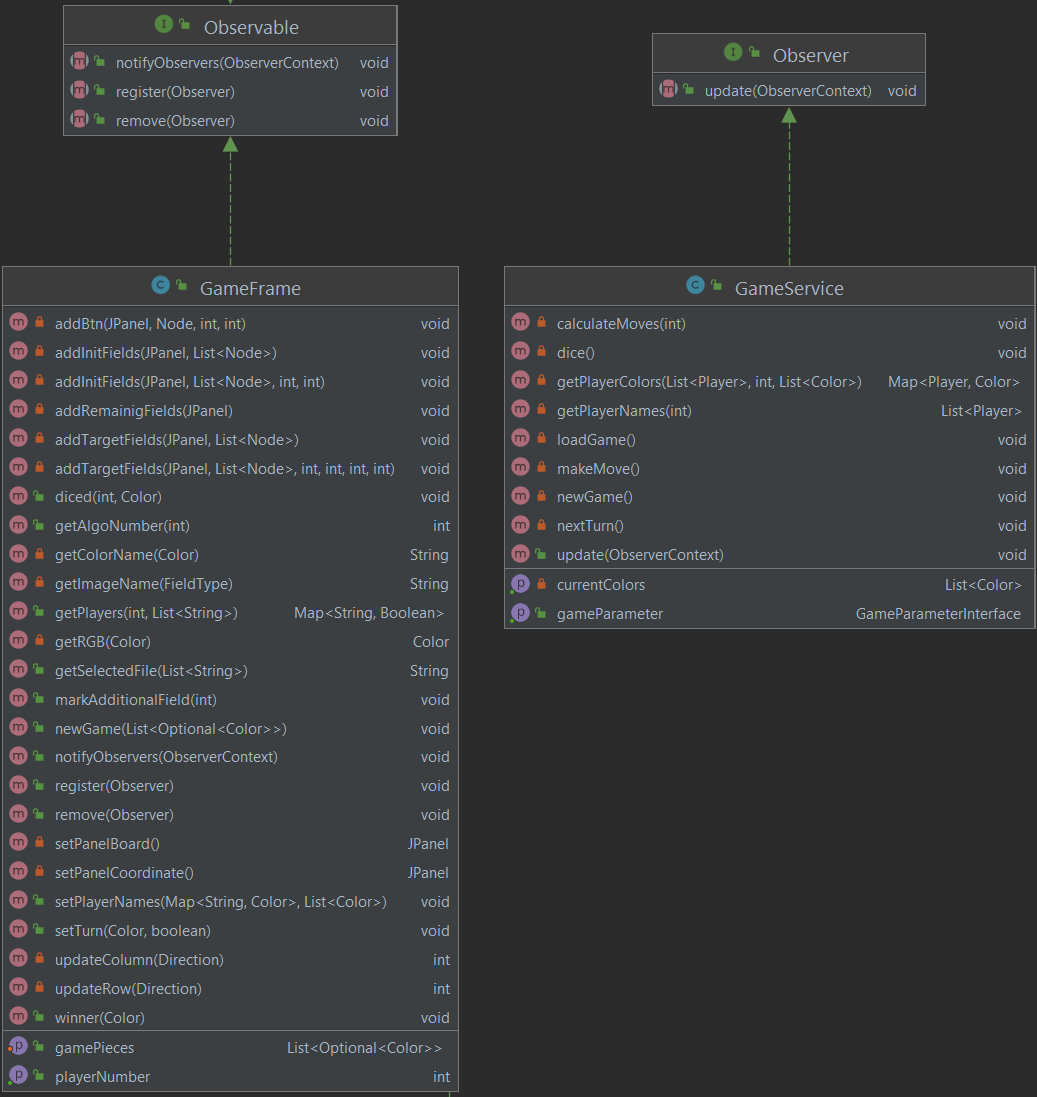
\includegraphics[scale=1]{grasp1}}
\caption{Positiv-Beispiel GRASP [Eigene Darstellung aus \emph{IntelliJ}]}
\label{fig:grasp1}
\end{figure}

\newpage
\subsubsection{Negativ-Beispiel}
\noindent Eine starke Kopplung liegt zwischen der \enquote{Algorithm}- Klasse und der \enquote{AbstractControl\-Mechnism}-Klasse vor. Erstere berechnet einen Zug, der nicht durch einen Benutzer ausgeführt wird -- wenn also ein Benutzer gegen den Algorithmus spielt. Die \enquote{AbstractControl\-Mechnism}-Klasse ruft die Zugberechnung auf. Die Klasse ist abstrakt, da der Aufruf für ein 4-Personen- oder ein 6-Personen-Spielfeld gleichermaßen gilt. 

Eine starke Kopplung liegt vor, da hier auf die konkrete \enquote{Algorithm}- Klasse zuge\-griffen wird. Die Kopplung könnte man durch die Implementierung einer Algorithm-Schnittstelle lockern. Dadurch könnten auch verschiedene Algorithmen implementiert werden.

\begin{figure}[htbp]
\centering
\centerline{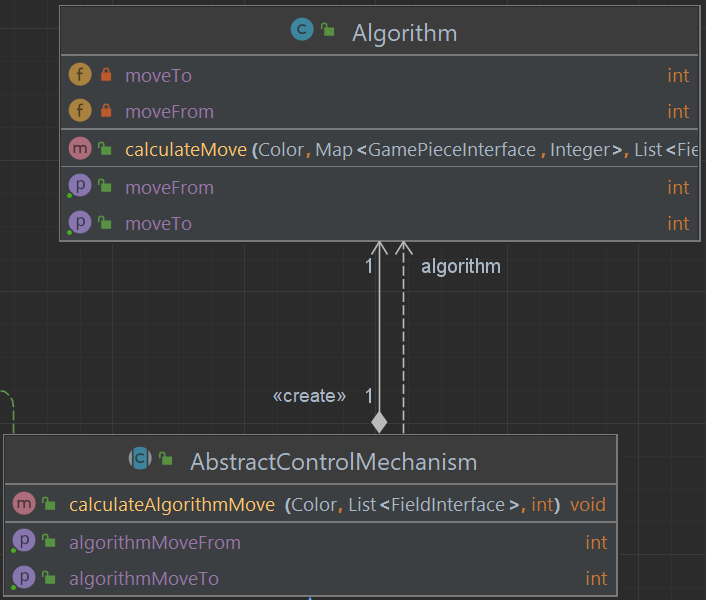
\includegraphics[scale=.6]{grasp2}}
\caption{Negativ-Beispiel GRASP [Eigene Darstellung aus \emph{IntelliJ}]}
\label{fig:grasp2}
\end{figure}

\newpage
\section{Analyse GRASP: Hohe Kohäsion (2P)}
\emph{[eine Klasse als positives Beispiel hoher Kohäsion; UML Diagramm und Begründung, warum die
Kohäsion hoch ist]}

\noindent Die Kohäsion erhöht sich, je mehr Verantwortlichkeiten und Teilaufgaben in andere Klassen ausgelagert sind. Ein Beispiel für hohe Kohäsion wäre hier der dem Spielfeld unterliegende Graph.

\todo{Bild}

\noindent In der \enquote{Graph}-Klasse wird der Graph aufgebaut. Hierzu wurden aber nicht alle Verantwortlichkeiten in dieser Klasse belassen, sondern in vier weitere Klassen ausgelagert.

\begin{itemize}
    \item Die \enquote{Node}-Klasse stellt einen Knoten dar und enthält den Feldtyp (Siehe \enquote{FieldType}) dieses Knotens und die ausgehenden Kanten (Siehe \enquote{Edge})
    \item Das \enquote{FieldType}-Enum gibt den Feldtyp an. Das kann ein neutrales Feld sein oder zum Beispiel ein rotes Startfeld oder ein gelbes Zielfeld.
    \item Die \enquote{Edge}-Klasse enthält den Zielknoten, die Richtung (Siehe \enquote{Direction}) und die Information, ob es ein Default-Kante ist. Letzteres bedeutet, dass die Kante von allen Spielfiguren befahren werden kann. Dies ist zum Beispiel bei der Kante zu den Zielfeldern der jeweiligen Farben nicht der Fall.
    \item Das \enquote{Direction}-Enum gibt an, in welche Richtung die Kante geht.
\end{itemize}

\newpage
\section{DRY (2P)}
\emph{[ein Commit angeben, bei dem duplizierter Code/duplizierte Logik aufgelöst wurde; Code-Beispiele
(vorher/nachher); begründen und Auswirkung beschreiben]}

\noindent Die Klasse \enquote{GraphUtilities} wurde hinzugefügt, da die jetzt enthaltenen vier Methoden früher von den drei Klassen \enquote{Graph}, \enquote{AbstractBoard} und \enquote{ControlMechanismFour} jeweils extra implementiert wurden und sich der Code dadurch dupliziert hat. Das Ergebnis:

\begin{figure}[htbp]
\centering
\centerline{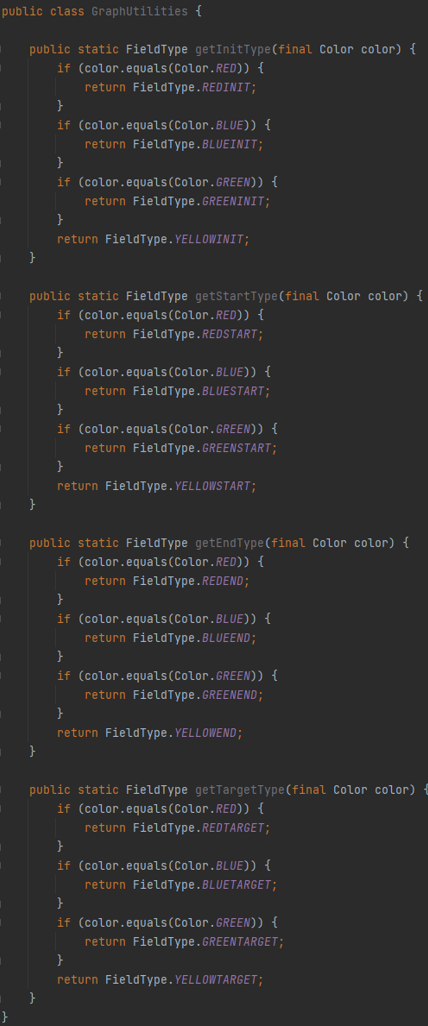
\includegraphics[scale=.6]{dry1}}
\caption{DRY [Eigene Darstellung aus \emph{IntelliJ}]}
\label{fig:dry1}
\end{figure}

\noindent In der \enquote{Graph}-Klasse waren früher alle vier Methoden, in der \enquote{AbstractBoard}-Klasse war nur die \enquote{getInitType}-Methode und in der \enquote{ControlMechanismFour}-Klasse waren ebenfalls alle vier Methoden vorhanden. Der Unterschied zum jetzigen Stand besteht darin, dass die Methoden mittlerweile statisch gemacht worden sind. Da sich innerhalb der Methode nichts verändert hat, sei hier der frühere Stand nicht als Codebeispiel aufgezeigt.

Positiv ist, dass sich der Code durch das Eliminieren von Duplikaten reduziert hat. Außerdem ist aus den einzelnen Klassen Code, der nicht zu deren Verantwortlichkeiten gezählt hat, herausgenommen worden. 

Die Klasse \enquote{GraphUtilities} existierte bis zu dem Commit \enquote{\texttt{Removed duplicated code to GraphUtilities}}.
%%%%%%%%%%%%%%%%%%%%%%%%%%%%%%%%%%%%%%%%%%%%%%%%%%%%%%%%%%%%%%%%%%%%%%%%%%%%%%%%%%%%%%%%%%%%%%%
%% Description:       Programmentwurf advanced software engineering
%% Author:      Manuel Berg, m.berg@enbw.com
%%  -*- coding: utf-8 -*-
%%%%%%%%%%%%%%%%%%%%%%%%%%%%%%%%%%%%%%%%%%%%%%%%%%%%%%%%%%%%%%%%%%%%%%%%%%%%%%%%%%%%%%%%%%%%%%%

\titlespacing*{\chapter}{0pt}{-30mm}{10pt}
\titleformat{\chapter}[display]
  {\normalfont\bfseries}{}{10pt}{\Huge\thechapter.\quad}
  
\chapter{Unit Tests (8P)}
\pagestyle{scrheadings}
\clearscrheadfoot
\pagenumbering{arabic}
\setcounter{page}{20}
\ofoot[\pagemark]{\pagemark}
%\ohead[\headmark]{\headmark}
\onehalfspacing

\section{10 Unit Tests (2P)}
\emph{[Nennung von 10 Unit-Tests und Beschreibung, was getestet wird]}

\begin{table}[htbp]
\centering
\centerline{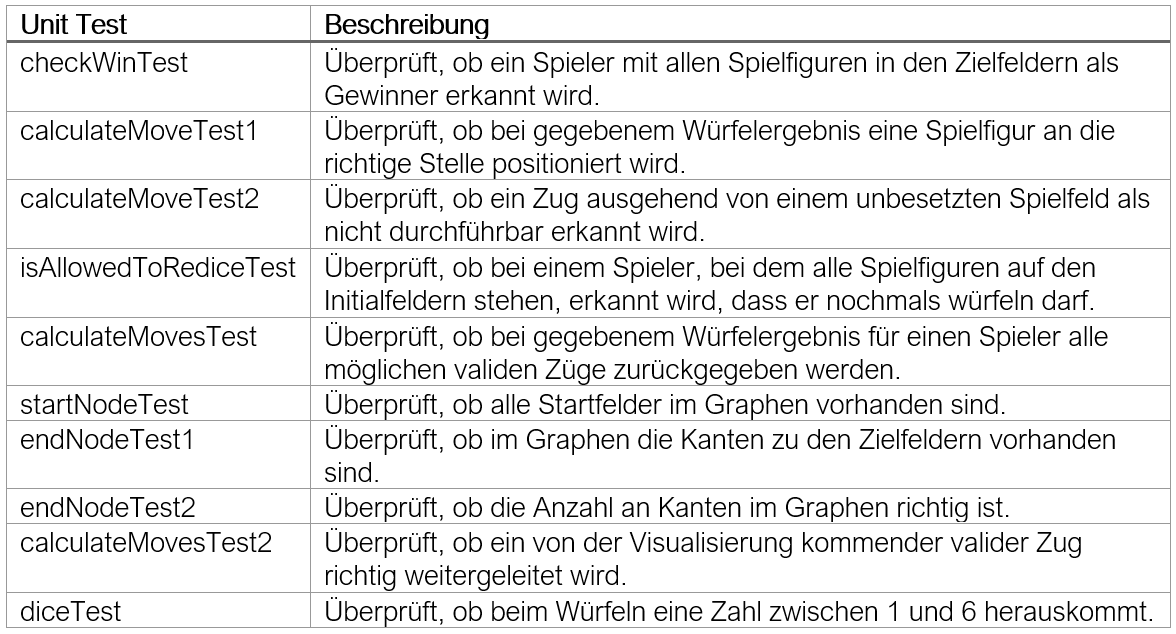
\includegraphics[scale=.55]{unitteststable}}
\caption{10 Unit Tests}
\label{tab:unitteststable}
\end{table}

\section{ATRIP: Automatic (1P)}
\emph{[Begründung/Erläuterung, wie ‘Automatic’ realisiert wurde]}
\vspace{.4cm}

\noindent Die Tests sind einfach auszuführen, denn es reicht auf dem Ordner, in dem alle Tests enthalten sind, das Starten aller Tests auszuwählen. Ein anderen Weg wäre das Ausführen des Befehls \textbf{\texttt{mvn clean test}}. Außerdem müssen bei keinem Test Daten manuell eingegeben werden. Somit laufen alle Tests automatisch ab. Des Weiteren überprüfen sich alle Tests selbst und geben als Ergebnis entweder bestanden oder fehlgeschlagen zurück.

\newpage
\section{ATRIP: Thorough (1P)}
\emph{[Code Coverage im Projekt analysieren und begründen]}
\vspace{.4cm}

\noindent Die Code Coverage im Projekt ist leider eher dürftig. Es wurden zwar die Kernfunktionen mit Tests abgedeckt, aber dennoch fehlen auch einige Aspekte, die wir als notwendig bezeichnen würden. Zum Beispiel gibt es keinerlei Tests zur GUI. Diese wurde nur händisch getestet.

Bei den Tests wurden einmal die möglichen Aktionen auf dem Spielbrett betrachtet. Hierzu zählen fünf ersten Tests aus der \hyperref[tab:unittesttable]{vorherigen Tabelle}. Außerdem wurde die dem Spielbrett zugrundeliegende Struktur, also der darunterliegende Graph, getestet. Hierbei sind aber auch nur cica 10\% des fertigen Graphen überprüft worden. Da dieser Graph zur Validierung von Zügen beisteuert ist dies eine kritische Stelle, die nicht mit Tests abgedeckt ist. Zum Schluss wurde dann noch der \enquote{GameService} mithilfe dreier Mocks getestet. Aber auch hier fehlt zum Beispiel die Überprüfung, ob ein neues Spiel richtig aufgebaut wird.

Bei der Erstellung der Tests wurde der Fokus auf die Kernfunktionalitäten gelegt. Es wurde aber beim Auftritt eines Fehlers dieser im Code verbessert und nicht direkt ein Test geschrieben. Zukünftig sollte das anders gehandhabt und auch direkt das Umfeld des Fehlers betrachtet werden.

\newpage
\section{ATRIP: Professional (1P)}
\emph{[jeweils 1 positves und negatives Beispiele zu \enquote{Professional}; jeweils Code-Beispiel, Analyse und
Begründung, was professionell/nicht professionell an den Beispielen ist]}

\begin{figure}[htbp]
\centering
\centerline{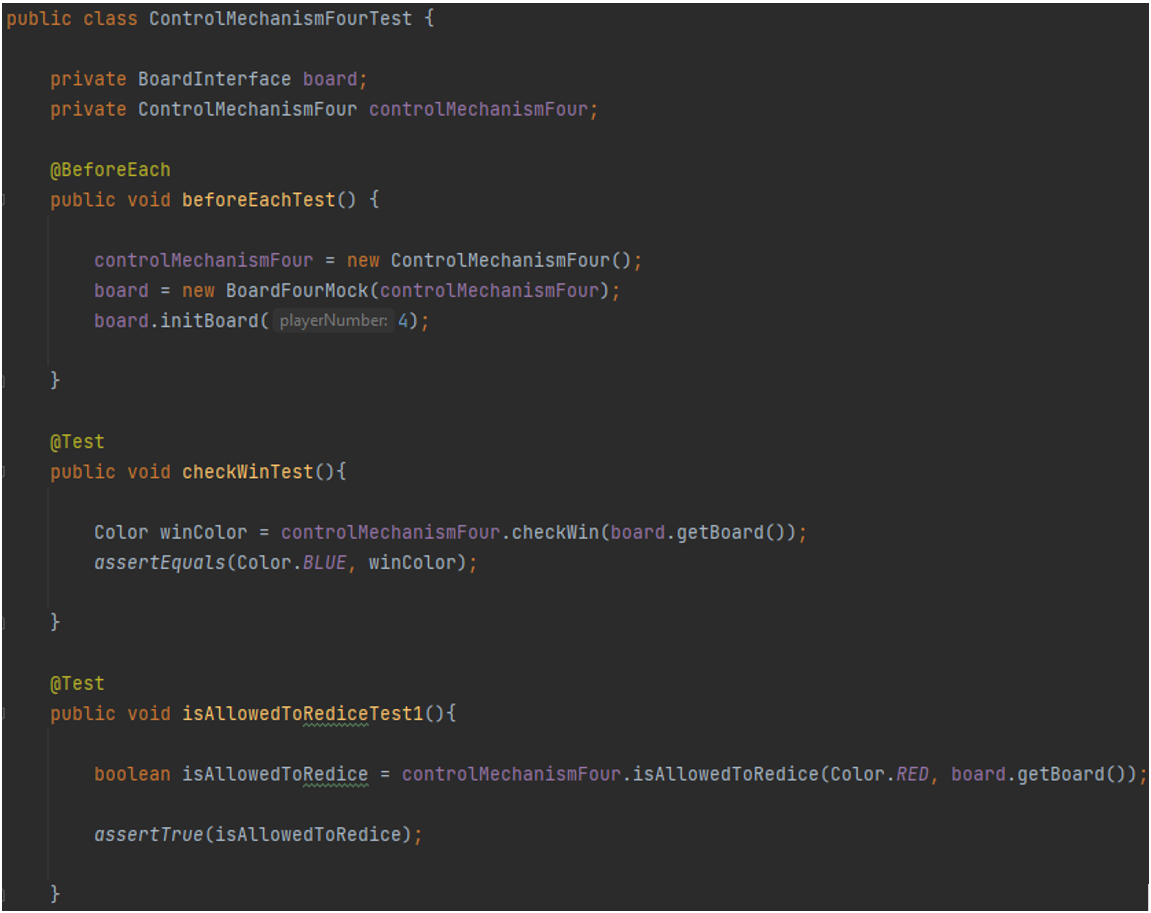
\includegraphics[scale=.5]{professional}}
\caption{Positiv-Beispiel Professional [Eigene Darstellung aus \emph{IntelliJ}]}
\label{fig:professional}
\end{figure}

\noindent Hier ist ein positives Beispiel zu \enquote{Professional} zu sehen. Es wird ein Mock für das Spielbrett eingesetzt. In der Testklasse werden verschiedene Aktionen beziehungsweise Funktionalitäten auf dem Spielbrett getestet. Hierbei wird der Code in der \enquote{beforeEachTest}-Methode wiederverwendet, was für \enquote{Professional} spricht. Hierdurch werden auch Fehlerquellen verkleinert, denn beispielsweise bei Änderungen muss hier nur eine Stelle im Code bedacht werden. Dies spricht auch für eine gute Code-Qualität.

\newpage

\begin{figure}[htbp]
\centering
\centerline{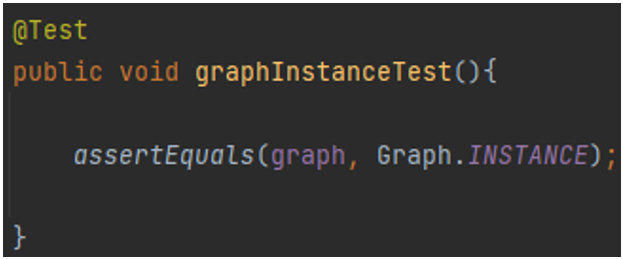
\includegraphics[scale=.5]{notprofessional}}
\caption{Negativ-Beispiel Professional [Eigene Darstellung aus \emph{IntelliJ}]}
\label{fig:notprofessional}
\end{figure}

\noindent Dieser Test überprüft, ob es tatsächlich nur eine Graph-Instanz gibt. Das ist aber sinnlos und ein Negativ-Beispiel zu \enquote{Professional}, da der Graph ein Singleton ist und somit nur eine Instanz existiert. 

\section{Fakes und Mocks (1P)}
\emph{[Analyse und Begründung des Einsatzes von 2 Fake/Mock-Objekten; zusätzlich jeweils UML
Diagramm der Klasse]}

\subsubsection{BoardFourMock}
\noindent Dieses Mock ist stellvertretend für ein Spielbrett. Dabei wurden nur die notwendigen Funktionalitäten implementiert. Das heißt, es gibt einen festen Spielstand der sozusagen \enquote{initialisiert} wird. Bei diesem Spielstand wurden absichtlich die Spielfiguren so gestellt, dass die möglichen Aktionen gut getestet werden können. Zum Beispiel ist die Farbe Blau im Ziel und somit kann die Funktion, ob jemand gewonnen hat, überprüft werden. Ein anderen Beispiel ist, dass Rot noch auf der Startposition steht und somit überprüft werden kann, ob Rot auch dreimal würfeln darf.

\begin{figure}[htbp]
\centering
\centerline{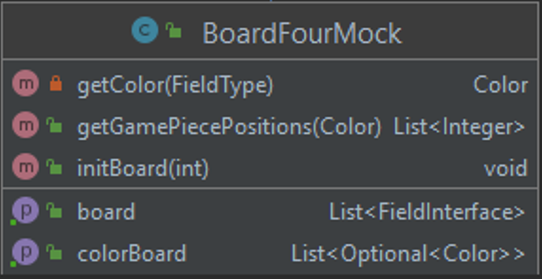
\includegraphics[scale=.5]{boardfourmock}}
\caption{BoardFourMock [Eigene Darstellung aus \emph{IntelliJ}]}
\label{fig:boardfourmock}
\end{figure}


\newpage
\subsubsection{GameFrameMock}
\noindent Das Mock \enquote{GameFrameMock} ist stellvertretend für die GUI da. Um den \enquote{GameService} ohne Abhängigkeiten testen zu können, wurden durch dieses Mock die minimal notwendigen Funktionalitäten geboten. Zum Beispiel konnte ohne die große GUI-Komponente mit einem akzeptablen Aufwand getestet werden, ob ein von der Visualisierung kommender valider Zug richtig weitergeleitet wird.

\begin{figure}[htbp]
\centering
\centerline{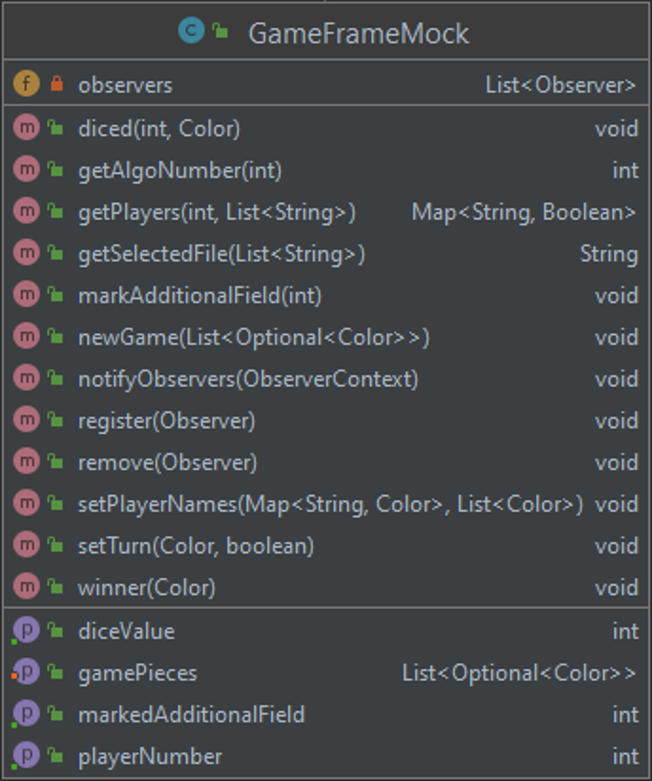
\includegraphics[scale=.5]{gameframemock}}
\caption{GameFrameMock [Eigene Darstellung aus \emph{IntelliJ}]}
\label{fig:gameframemock}
\end{figure}

\newpage
\titlespacing*{\chapter}{0pt}{-30mm}{10pt}
\titleformat{\chapter}[display]
  {\normalfont\bfseries}{}{10pt}{\Huge\thechapter.\quad}
  
\chapter{Domain Driven Design (8P)}
\pagestyle{scrheadings}
\clearscrheadfoot
\pagenumbering{arabic}
\setcounter{page}{25}
\ofoot[\pagemark]{\pagemark}
%\ohead[\headmark]{\headmark}
\onehalfspacing

\section{Ubiquitous Language (2P)}
\emph{[4 Beispiele für die Ubiquitous Language; jeweils Bezeichung, Bedeutung und kurze Begründung,
warum es zur Ubiquitous Language gehört]}

\begin{table}[htbp]
\centering
\centerline{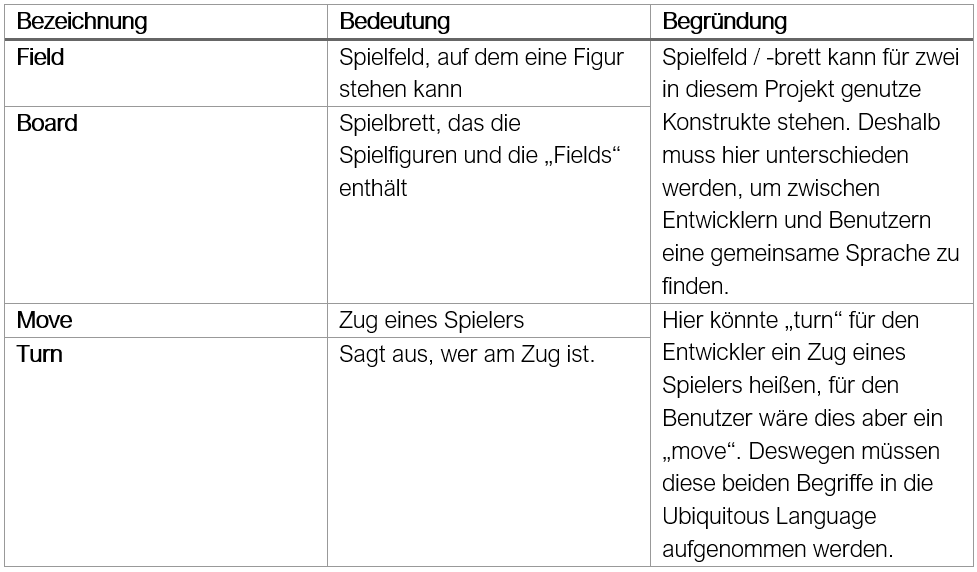
\includegraphics[scale=.7]{ubiquitous}}
\caption{4 Beispiele für die Ubiquitous Language}
\label{tab:ubiquitous}
\end{table}

% \begin{table}[htbp]
% \centering
%     \begin{tabular}{|l|l|l|}
%         \hline
%         \textbf{Bezeichnung} & \textbf{Bedeutung} & \textbf{Begründung} \\ \hline
%         ~         & ~          & ~  \\ \hline
%         ~         & ~          & ~  \\ \hline
%         ~         & ~          & ~  \\ \hline
%         ~         & ~          & ~  \\ 

%         \hline
%     \end{tabular}
%     \label{Tab:ddd_examples}
%     \caption{4 Beispiele für die Ubiquitous Language}
% \end{table}

\newpage

\section{Repositories (1,5P)}
\emph{[UML, Beschreibung und Begründung des Einsatzes eines Repositories; falls kein Repository
vorhanden: ausführliche Begründung, warum es keines geben kann/hier nicht sinnvoll ist]}

\vspace{.4cm}

\noindent Das Repository wird durch die Klasse \enquote{GameIO} repräsentiert und bietet Zugriff auf persistenten Speicher. Außerdem wird die konkret verwendete Speichertechnologie vor dem Domain Code verborgen. In unserem Beispiel ist es das Abspeichern und Laden von Spielständen, was mithilfe von JSON umgesetzt wird. Dadurch kann ein Spiel unterbrochen und später fortgesetzt werden.

\begin{figure}[htbp]
\centering
\centerline{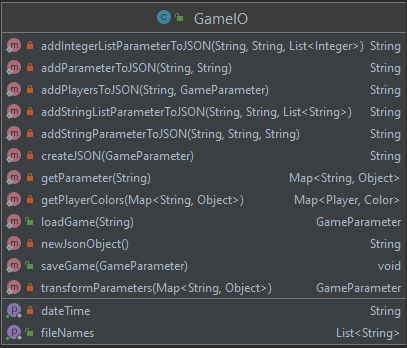
\includegraphics[scale=.6]{repo}}
\caption{Repository [Eigene Darstellung aus \emph{IntelliJ}]}
\label{fig:repo}
\end{figure}

\newpage

\section{Aggregates (1,5P)}
\emph{[UML, Beschreibung und Begründung des Einsatzes eines Aggregates; falls kein Aggregate
vorhanden: ausführliche Begründung, warum es keines geben kann/hier nicht sinnvoll ist]}

\begin{figure}[htbp]
\centering
\centerline{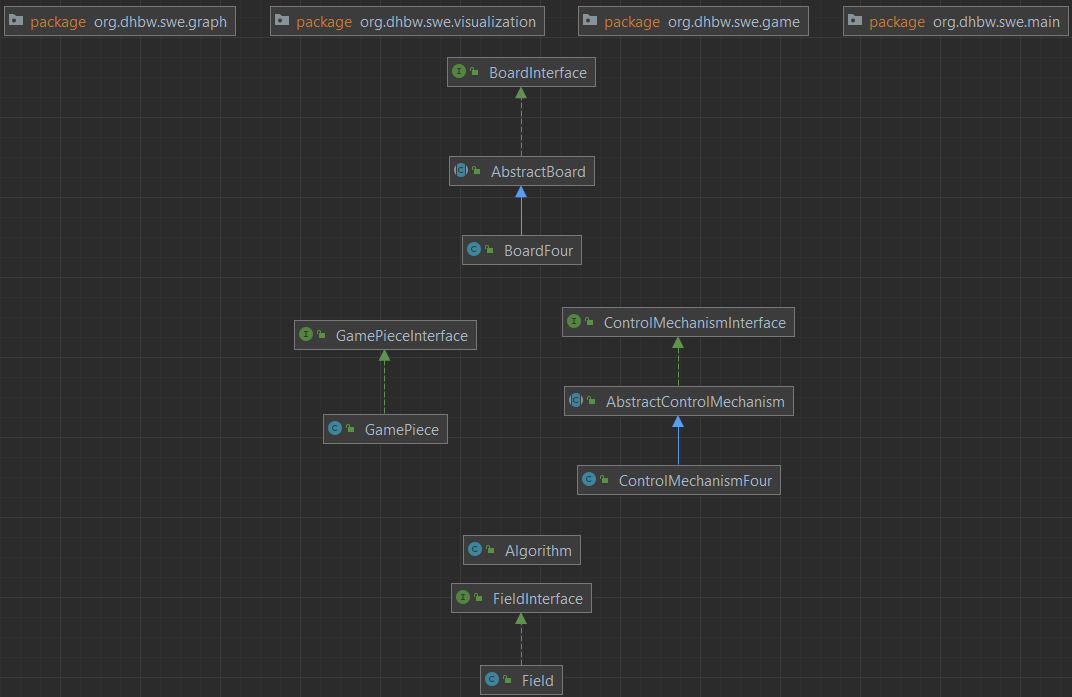
\includegraphics[scale=.6]{aggregat}}
\caption{Aggregate [Eigene Darstellung aus \emph{IntelliJ}]}
\label{fig:aggregat}
\end{figure}

\noindent Die in \hyperref[fig:aggregat]{Abbildung 6.2} dargestellten Klassen gehören zu einem Aggregat. Dies ist eine gemeinsam verwaltete Einheit und ist innerhalb seiner Grenzen konsistent. Durch diese Konsistenzgrenze war es sinnvoll, das Aggregat für das Spielbrett einzusetzen, da beispielsweise auch die Züge stets konsistent sein müssen. Als Aggregatswurzel fungiert das \enquote{BoardInterface}. Dieses kontrolliert alle Zugriffe auf das Aggregat. Wenn eines der vier oben dargestellten Packages Änderungen am Spielbrett vornehmen möchte, geht dies nur über die Aggregatswurzel. 

\section{Entities (1,5P)}
\emph{[UML, Beschreibung und Begründung des Einsatzes einer Entity; falls keine Entity vorhanden:
ausführliche Begründung, warum es keines geben kann/hier nicht sinnvoll ist]}

\begin{figure}[htbp]
\centering
\centerline{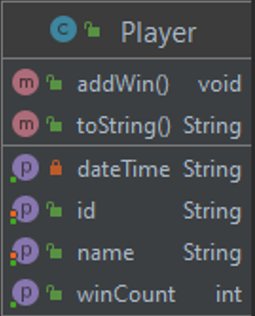
\includegraphics[scale=.6]{entities}}
\caption{Entitiy Player [Eigene Darstellung aus \emph{IntelliJ}]}
\label{fig:entities}
\end{figure}

\noindent Jeder Player hat eine eindeutige Identität. Alle Spieler, die jemals teilgenommen haben, werden in einer JSON-Datei gespeichert und durch die \enquote{id} identifiziert. Dadurch kann auch die insgesamte Anzahl an Gewinnen abgespeichert werden. Anhand dieser sich über die Zeit verändernden Zahl \enquote{winCount} ist zu erkennen, dass der \enquote{Player} veränderliche Eigenschaften und einen Lebenszyklus hat. 

Aufgrund der Anforderungen waren hier eine Identität und veränderliche Eigenschaften notwendig. Da dies Merkmale einer Entity sind war es hier sinnvoll den \enquote{Player} als eine solche zu implementieren.

\newpage
\section{Value Objects (1,5P)}
\emph{[UML, Beschreibung und Begründung des Einsatzes eines Value Objects; falls kein Value Object
vorhanden: ausführliche Begründung, warum es keines geben kann/hier nicht sinnvoll ist]}

\begin{figure}[htbp]
\centering
\centerline{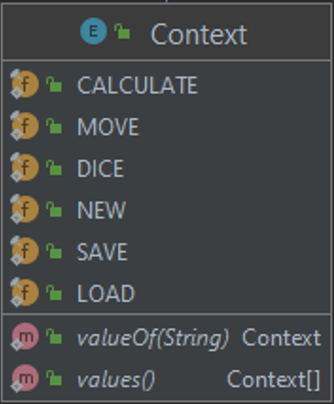
\includegraphics[scale=.6]{valueobjects}}
\caption{Enum als Value Object [Eigene Darstellung aus \emph{IntelliJ}]}
\label{fig:valueobjects}
\end{figure}

\noindent Ein Enum hat keine Identität, was auch auf Value Objects zutrifft. Außerdem sind Value Objects gleich, wenn sie denselben Wert haben. Dies lässt sich einfach durch \textbf{\texttt{Context.DICE.equals(Context.DICE)}}. Da dies wahr ist, trifft auch dieser Aspekt des ValueObject auf das \enquote{Context}-Enum zu. Des Weiteren haben ValueObjects keinen Lebenszyklkus, was auch hier passt. Da das \enquote{Context}-Enum keine Instanzvariablen besitzt ist es auch unveränderlich. Das bedeutet nicht alle Enums sind Value Objects, aber das hier gezeigte Enum ist eines.

% \begin{figure}[htbp]
% \centering
% \centerline{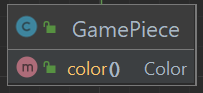
\includegraphics[scale=.6]{valueobject}}
% \caption{Value Object [Eigene Darstellung aus \emph{IntelliJ}]}
% \label{fig:valueobject}
% \end{figure}

% \noindent Ein Value Object ist hier eine Spielfigur. Diese hat als Eigenschaft nur die Farbe, welche über den gesamten Zeitraum hinweg unveränderlich bleibt. Die Änderung der Farbe ist nur durch die Konstruktion eines neuen Objektes möglich. Die Spielfigur besitzt keine eigene Identität und es ist auch kein Lebenszyklus erkennbar.

% Bezüglich des \enquote{GamePiece} sind das Überschreiben von \enquote{equals()} und \enquote{hashCode()} sowie die weiteren Vorgaben aus der Vorlesung zur Implementierung von Value Objects in Java beachtet worden.

\newpage
\titlespacing*{\chapter}{0pt}{-30mm}{10pt}
\titleformat{\chapter}[display]
  {\normalfont\bfseries}{}{10pt}{\Huge\thechapter.\quad}
  
\chapter{Refactoring (8P)}
\pagestyle{scrheadings}
\clearscrheadfoot
\pagenumbering{arabic}
\setcounter{page}{29}
\ofoot[\pagemark]{\pagemark}
%\ohead[\headmark]{\headmark}
\onehalfspacing

\section{Code Smells (2P)}
\emph{[jeweils 1 Code-Beispiel zu 2 unterschiedlichen Code Smells aus der Vorlesung; jeweils Code-Beispiel
und einen möglichen Lösungsweg bzw. den genommen Lösungsweg beschreiben (inkl. (Pseudo-)Code)]}

\subsubsection{Long Method}
\noindent Dieser Code Smell war in der \enquote{calculateTurn}-Methode in der \enquote{ControlMechanismFour}-Klasse enthalten. Wie in \hyperref[fig:longmethod]{Abbildung 7.1} ersichtlich, ist die Methode viel zu lang. Zusätzlich mussten noch Kommentare eingefügt werden, dass die Methode überhaupt einigermaßen verständlich ist. 

Nach der Eliminierung des Code Smells sind nur noch die drei logischen Möglichkeiten nach den Spielregeln in der Methode enthalten. Das eigentliche Berechnen der Züge ist ausgelagert. Durch die Methodennamen sind auch keine Kommentare mehr notwendig.

\begin{figure}[htbp]
\centering
\centerline{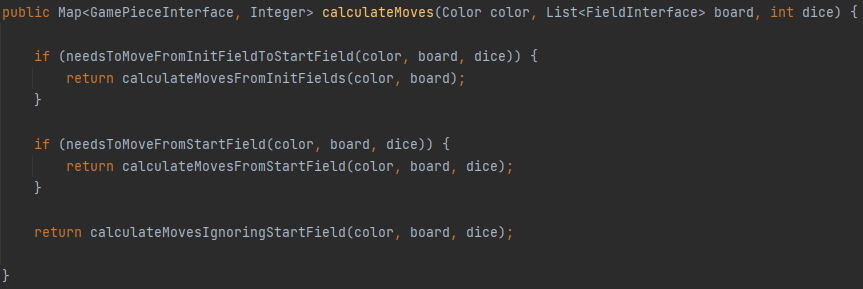
\includegraphics[scale=.5]{longmethodsolution}}
\caption{Eliminierung der Long Method [Eigene Darstellung aus \emph{IntelliJ}]}
\label{fig:longmethodsolution}
\end{figure}

\begin{figure}[htbp]
\centering
\centerline{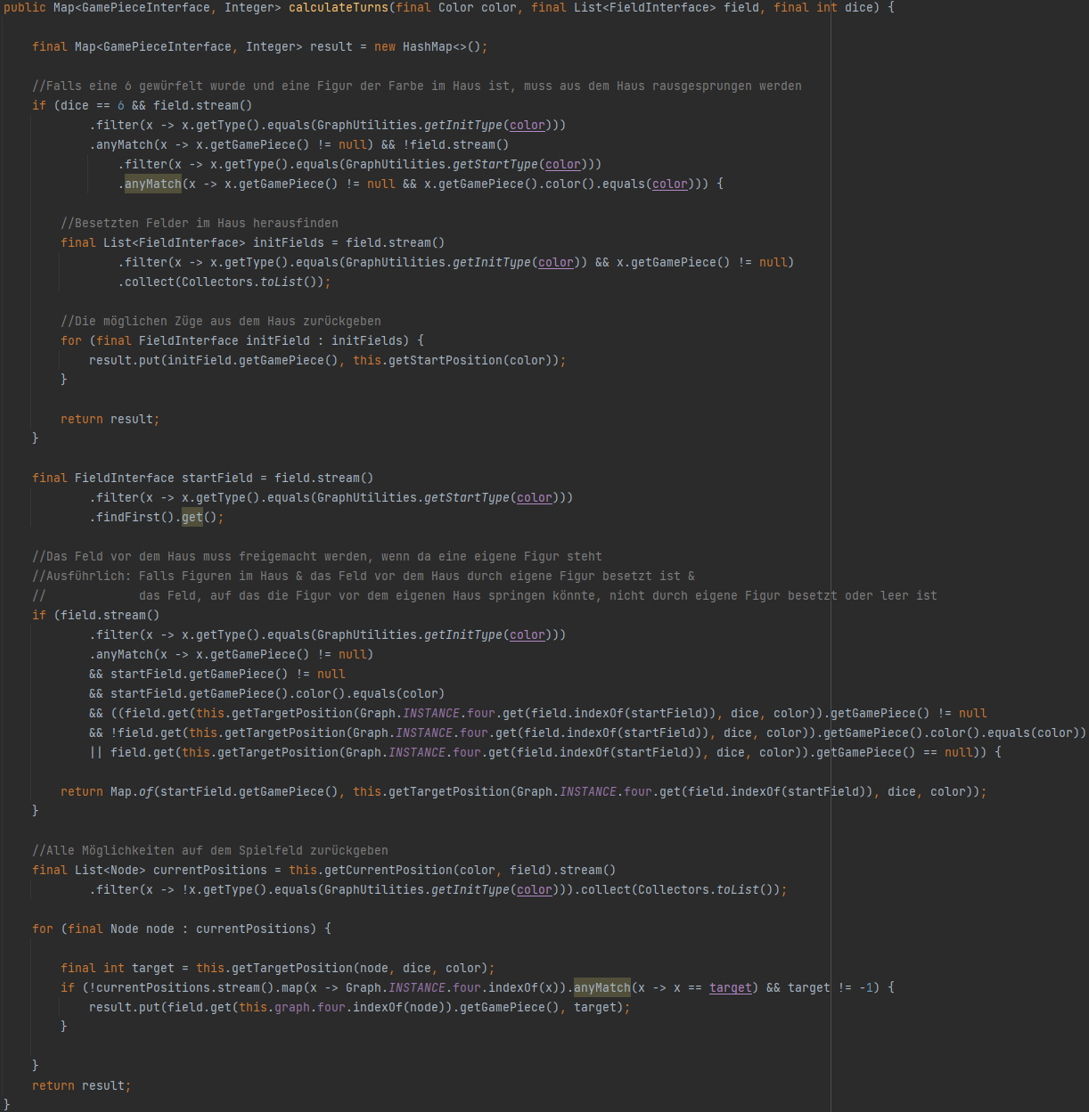
\includegraphics[scale=.65]{longmethod}}
\caption{Long Method [Eigene Darstellung aus \emph{IntelliJ}]}
\label{fig:longmethod}
\end{figure}

\newpage

\subsubsection{Switch-Statements}

\begin{figure}[htbp]
\centering
\centerline{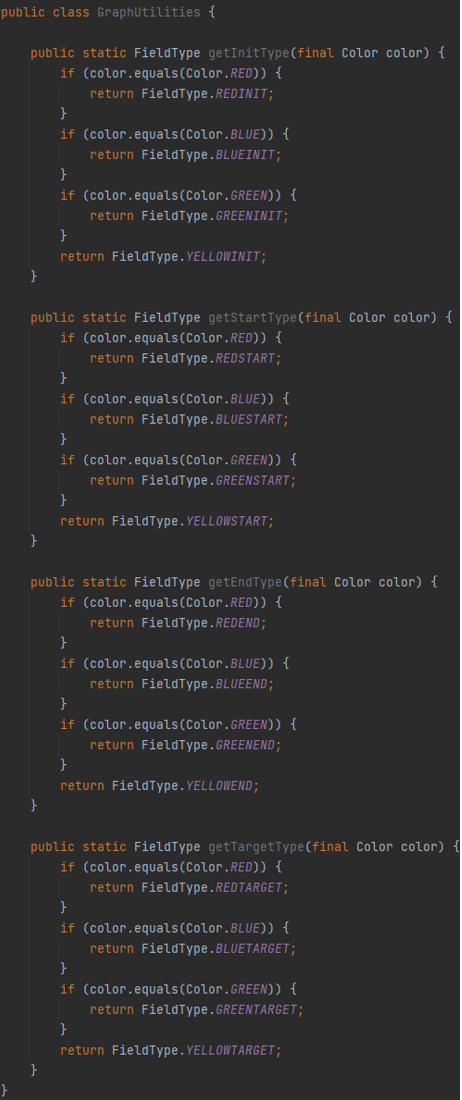
\includegraphics[scale=.55]{graphutilities}}
\caption{Switch-Statements [Eigene Darstellung aus \emph{IntelliJ}]}
\label{fig:graphutilities}
\end{figure}

\noindent Der Code-Smell bezieht sich auf die vier Methoden der \enquote{GraphUtilities}-Klasse (\hyperref[fig:graphutilities]{siehe Abbildung 7.3}). Der Switch-Statements Code Smell gilt auch hier, da die if-else-Statements einfach durch switch-Statements ersetzt werden können. Da sich diese Methoden alle um das \enquote{FieldType}-Enum drehen, wäre an dieser Stelle eine Implementierung der Methoden im Enum sinnvoller und würden den Code-Smell entfernen. 

\newpage
\noindent Das Enum wurde um fünf Instanzvariablen erweitert:

\begin{figure}[htbp]
\centering
\centerline{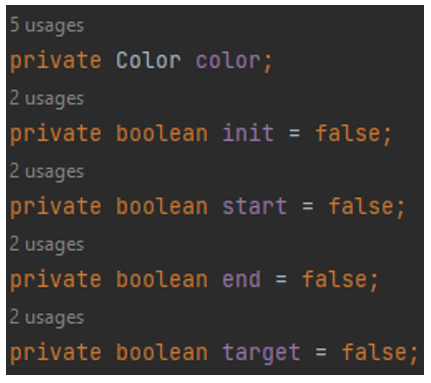
\includegraphics[scale=.55]{instanzvariablen}}
\caption{Erweiterung um fünf Instanzvariablen [Eigene Darstellung aus \emph{IntelliJ}]}
\label{fig:instanzvariablen}
\end{figure}

\noindent Außerdem wurden die vier Funktionalitäten aus den Graph-Utilities hinzugefügt, wie auf der nächsten Seite zu sehen ist.

\begin{figure}[htbp]
\centering
\centerline{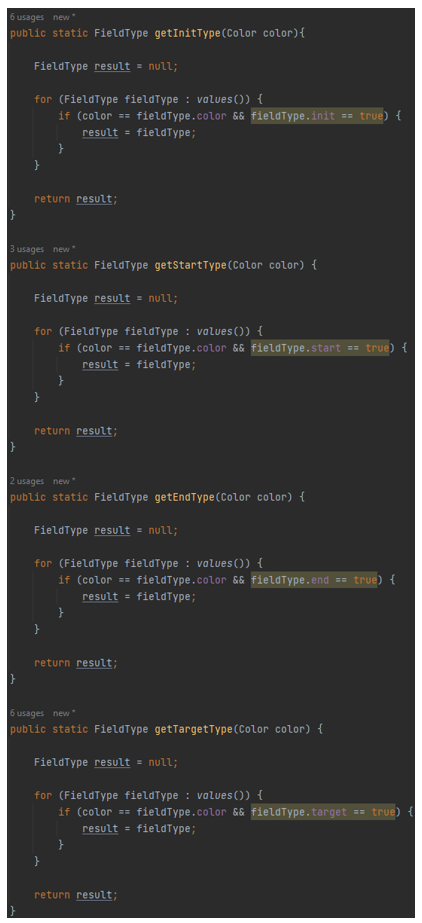
\includegraphics[scale=.8]{functionalities}}
\caption{Hinzufügen der vier Funktionalitäten [Eigene Darstellung aus \emph{IntelliJ}]}
\label{fig:funtionalities}
\end{figure}

\newpage
\section{2 Refactorings (6P)}
\emph{[2 unterschiedliche Refactorings aus der Vorlesung anwenden, begründen, sowie UML vorher/nachher
liefern; jeweils auf die Commits verweisen]}

\subsubsection{Extract Method}
\noindent Die Methode \enquote{saveGame} in der Klasse \enquote{GameIO} hat zuerst einen JSON-String erstellt und dann diesen mit dem aktuellen Zeitpunkt im Dateinamen abgespeichert. Beim Refactoring wurde hier einmal das Erstellen des JSON-Strings und das Generieren des aktuellen Zeitpunkts ausgelagert. Jetzt befindet sich nur noch der tatsächliche Abspeicherungsprozess in der Methode. Sichtbar war der alte Stand bis zum Commit \textbf{\texttt{aee0fe5f52b545c68111ffcfbef3e99b8f85caf8}} vom 27.05.2022.

\begin{figure}[htbp]
\centering
\centerline{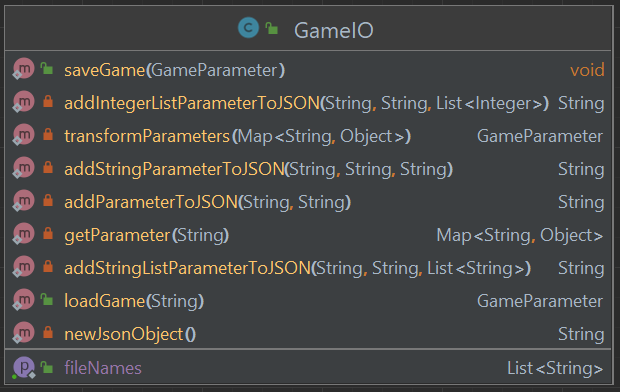
\includegraphics[scale=.45]{gameio1}}
\caption{Extract Method (vorher) [Eigene Darstellung aus \emph{IntelliJ}]}
\label{fig:gameio1}
\end{figure}

\begin{figure}[htbp]
\centering
\centerline{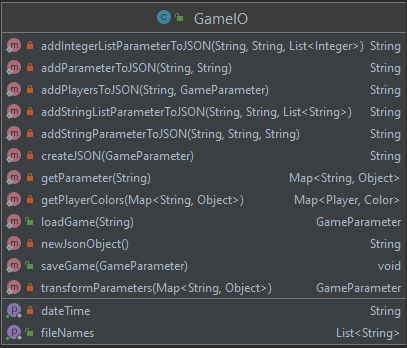
\includegraphics[scale=.5]{gameio2}}
\caption{Extract Method (nacher) [Eigene Darstellung aus \emph{IntelliJ}]}
\label{fig:gameio2}
\end{figure}

\newpage
\subsubsection{Rename Method}
\noindent Bei diesem Refactoring wurde auf die einheitliche Ubiquitous Language umgestellt. Dies ist zum Beispiel bei der \emph{CalculateMove}-Methode im \emph{ControlMechanismInterface} der Fall. Hier stand in den Argumenten statt \emph{board} der Begriff \emph{field}. Sichtbar war der alte Stand bis zum Commit \textbf{\texttt{aee0fe5f52b545c68111ffcfbef3e99b8f85caf8}} vom 27.05.2022.

\begin{figure}[htbp]
\centering
\centerline{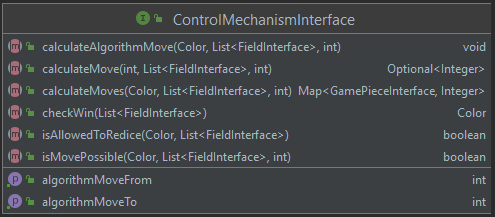
\includegraphics[scale=.6]{renamemethod}}
\caption{Rename Method [Eigene Darstellung aus \emph{IntelliJ}]}
\label{fig:renamemethod}
\end{figure}

\newpage
\titlespacing*{\chapter}{0pt}{-30mm}{10pt}
\titleformat{\chapter}[display]
  {\normalfont\bfseries}{}{10pt}{\Huge\thechapter.\quad}
  
\chapter{Entwurfsmuster (8P)}
\pagestyle{scrheadings}
\clearscrheadfoot
\pagenumbering{arabic}
\setcounter{page}{35}
\ofoot[\pagemark]{\pagemark}
%\ohead[\headmark]{\headmark}
\onehalfspacing

\emph{[2 unterschiedliche Entwurfsmuster aus der Vorlesung (oder nach Absprache auch andere) jeweils
sinnvoll einsetzen, begründen und UML-Diagramm]}

\subsubsection{Entwurfsmuster: Singleton (4P)}
\noindent Der Graph ist ein Singleton-Enum und liegt sozusagen unter dem Spielbrett. Er besteht aus Knoten und gerichteten Kanten und gibt somit die Struktur wieder. Da der Graph von mehrerer Teilen des Systems verwendet wird und sich nie ändert, ist es hier nicht notwendig mehrere Instanzen des Graphen zu haben. Deswegen haben wir uns an dieser Stelle für das Singleton-Pattern entschieden.

\begin{figure}[htbp]
\centering
\centerline{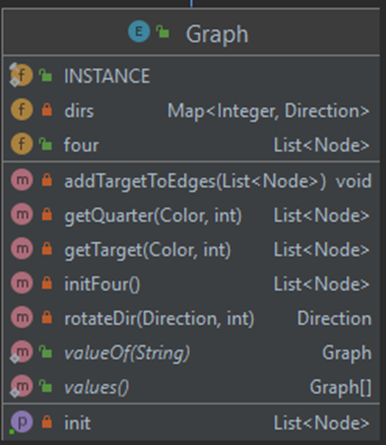
\includegraphics[scale=.5]{singleton}}
\caption{Graph als Singleton-Enum [Eigene Darstellung aus \emph{IntelliJ}]}
\label{fig:singleton}
\end{figure}

\newpage
\subsubsection{Entwurfsmuster: Observer-Pattern (4P)}
\noindent Das Observer-Pattern wurde eingesetzt, um eine lose Kopplung zwischen der Verwaltung des Spiels (\emph{GameService}-Klasse) und der Visualisierung (\emph{GameFrame}-Klasse) zu schaffen. Da die \emph{GameFrame}-Klasse mit dem Benutzer interagiert, muss dies an die \emph{GameService}-Klasse weitergeleitet werden. Ein direkter Methodenaufruf würde hier eine starke Kopplung schaffen und deshalb haben wir uns für das Observer-Pattern entschieden.

\begin{figure}[htbp]
\centering
\centerline{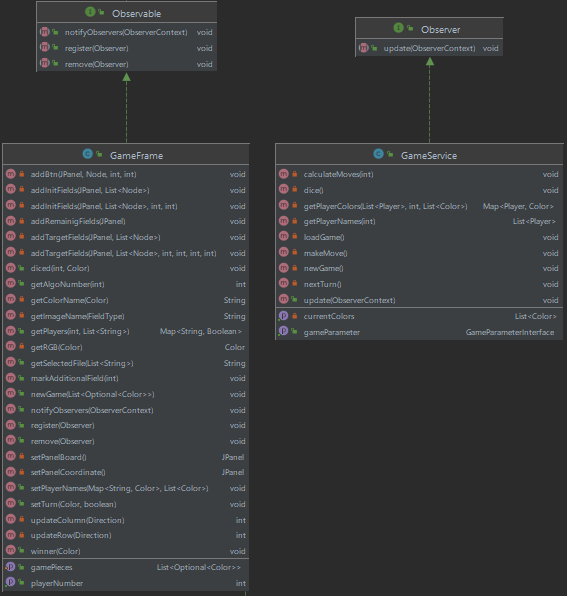
\includegraphics[scale=.7]{observer}}
\caption{Observer-Pattern [Eigene Darstellung aus \emph{IntelliJ}]}
\label{fig:oberver}
\end{figure}

\newpage
\titlespacing*{\chapter}{0pt}{-30mm}{10pt}
\titleformat{\chapter}[display]
  {\normalfont\bfseries}{}{10pt}{\Huge\thechapter.\quad}
  
\chapter{Anhang: Bedienungsanleitung}
\label{ch:anleitung}
\pagestyle{scrheadings}
\clearscrheadfoot
\pagenumbering{arabic}
\setcounter{page}{36}
\ofoot[\pagemark]{\pagemark}
%\ohead[\headmark]{\headmark}
\onehalfspacing

\noindent Zu Beginn eines Spiels wird zunächst die Anzahl an Spielern angegeben. Hierbei kann zwischen 2, 3 oder 4 ausgewählt werden.

\begin{figure}[htbp]
\centering
\centerline{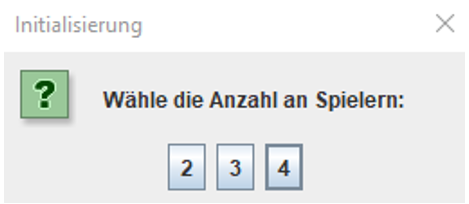
\includegraphics[scale=.5]{anleitung1}}
\caption{Auswahl der Spieleranzahl}
\label{fig:anleitung1}
\end{figure}

\noindent Nachdem die Spieleranzahl ausgewählt wurde, wird als nächstes die Anzahl der durch den Algorithmus gespielten Spielern ausgewählt. Es können bis zu 3 Spieler als Algorithmus initialisiert werden.

\begin{figure}[htbp]
\centering
\centerline{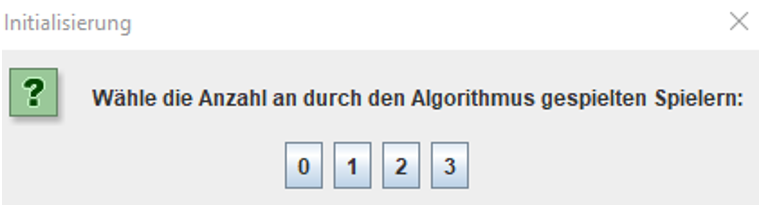
\includegraphics[scale=.5]{anleitung2}}
\caption{Auswahl der Anzahl an simulierten Spielern}
\label{fig:anleitung2}
\end{figure}

\noindent Im nächsten Schritt werden die nicht-algorithmischen Spieler festgelegt. Hierbei können Spielern deren Namen zugewiesen werden. Alternativ können auch bereits existierende Spieler ausgewählt werden. Im Folgenden wurde Spieler 1 als neuer Spieler unter dem Namen Nadine angelegt. Als Spieler 2 wurde ein bereits existierender Spieler ausgewählt.

\newpage

% \begin{figure}[htbp]
% \centering
% \centerline{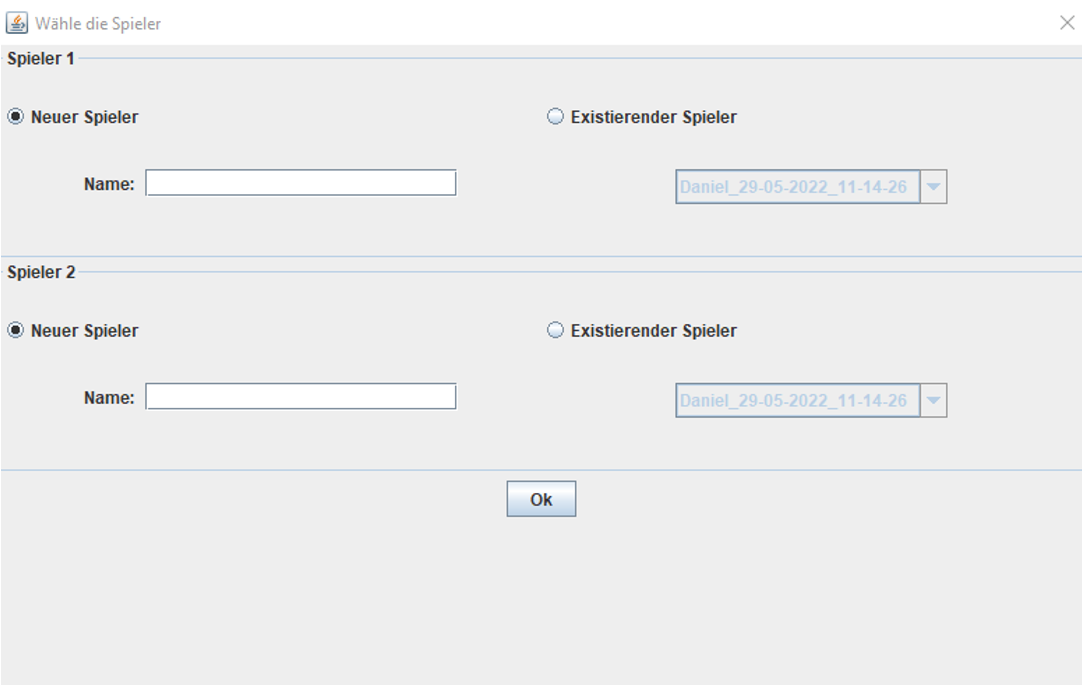
\includegraphics[scale=.6]{anleitung3}}
% \caption{Benennung der Spieler}
% \label{fig:anleitung3}
% \end{figure}

\begin{figure}[htbp]
\centering
\centerline{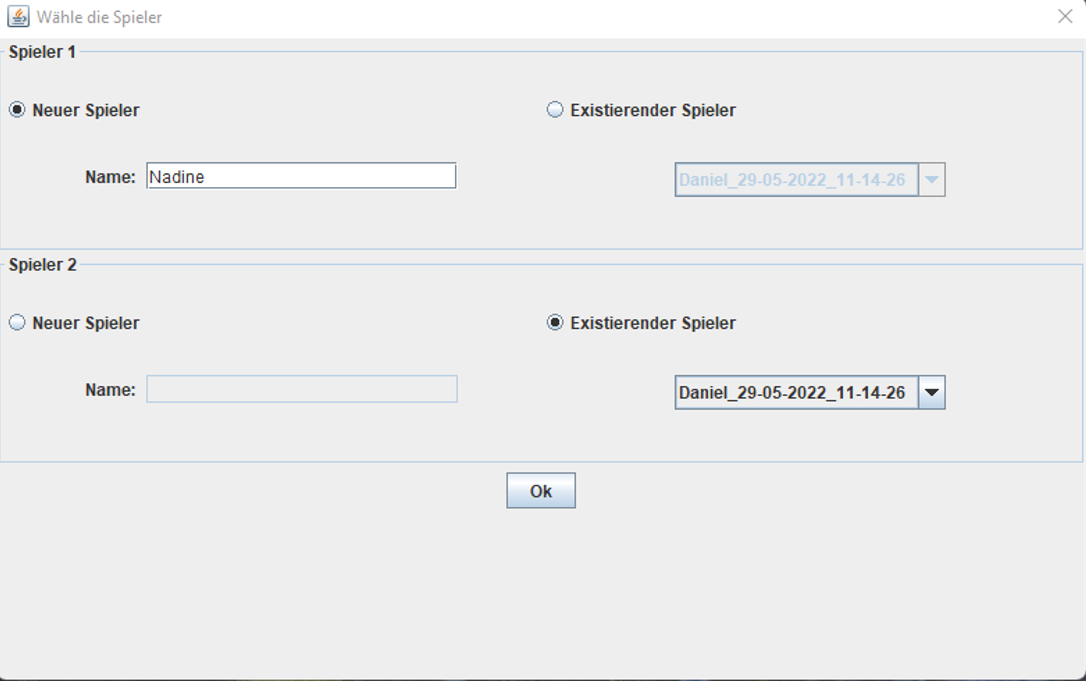
\includegraphics[scale=.6]{anleitung4}}
\caption{Benennung eines Spielers und Auswahl eines existierenden Spielers}
\label{fig:anleitung4}
\end{figure}

\noindent Nachdem Abschließend OK ausgewählt wurde beginnt das Spiel. Jeder Spieler erhält 4 Spielfiguren einer Farbe. Alle 4 Figuren stehen zu Beginn eines Spiels auf dem Feld A seiner Farbe. Die jeweiligen Spieler werden unterhalb des Spielfeldes mit Namen und ihrer jeweiligen Farbe angezeigt.

Die weißen Felder des Spielbretts stellen die Laufbahn C dar, die alle Spielfiguren zurücklegen müssen. Auf den jeweils farbigen Feldern auf der Laufbahn C beginnen die Spielfiguren ihren Weg über die weißen Felder. Auf der A-Feldern warten die Spielfiguren auf ihren Einsatz. Wer seine 4 Spielfiguren als erster in sein jeweiliges Ziel (Punkt D) gebracht hat, gewinnt das Spiel.

\newpage

\noindent Der Spieler, der an der Reihe ist, würfelt durch Klicken auf das Symbol \enquote{Fragezeichen in der Box} bei Punkt B. Wer keine Spielfigur auf der Laufbahn hat, weil alle Figuren geschlagen wurden oder zu Beginn des Spiels, darf dreimal würfeln. Die Spielfiguren, die auf den A-Feldern stehen, können nur mit einer \enquote{6} in das Spiel gebracht werden. Wird eine \enquote{6} gewürfelt, kann der Spieler selbst entscheiden mit welcher Figur er vom Startfeld A gehen möchte. Durch das Anklicken einer Figur wird diese ausgewählt und die Startposition auf der Laufbahn wird in Orange angezeigt. Wer eine \enquote{6} würfelt, hat nach seinem Zug einen weiteren Wurf frei. Erzielt er dabei wieder eine \enquote{6}, darf er nach dem Ziehen erneut würfeln. Bei einer \enquote{6} muss man eine neue Figur ins Spiel bringen, solange noch Spielfiguren auf dem eigenen A-Feldern stehen. Die neue Figur wird dann auf die Startposition der Laufbahn gestellt. Ist dieses Feld noch von einer anderen eigenen Spielfigur besetzt, muss diese Figur erst mit der \enquote{6} weitergezogen werden. Steht dagegen eine fremde Figur auf dem Feld, wird sie geschlagen. Wer eine \enquote{6} würfelt und keine Spielfigur mehr auf den B-Feldern hat, darf mit einer seiner Figuren auf der Laufbahn sechs Felder weiterziehen und dann noch einmal würfeln.

Eigene und fremde Figuren können übersprungen werden. Die besetzten Felder werden aber mitgezählt. Wer mehrere Spielfiguren auf der Laufbahn hat, kann sich aussuchen, mit welcher Figur er weiterzieht. Wer mit dem letzten Punkt seiner Augenzahl auf ein Feld tritt, das von einer fremden Spielfigur besetzt ist, schlägt diese Figur, welche wiederum automatisch zurück in den Startplatz gesetzt wird. 

\begin{figure}[htbp]
\centering
\centerline{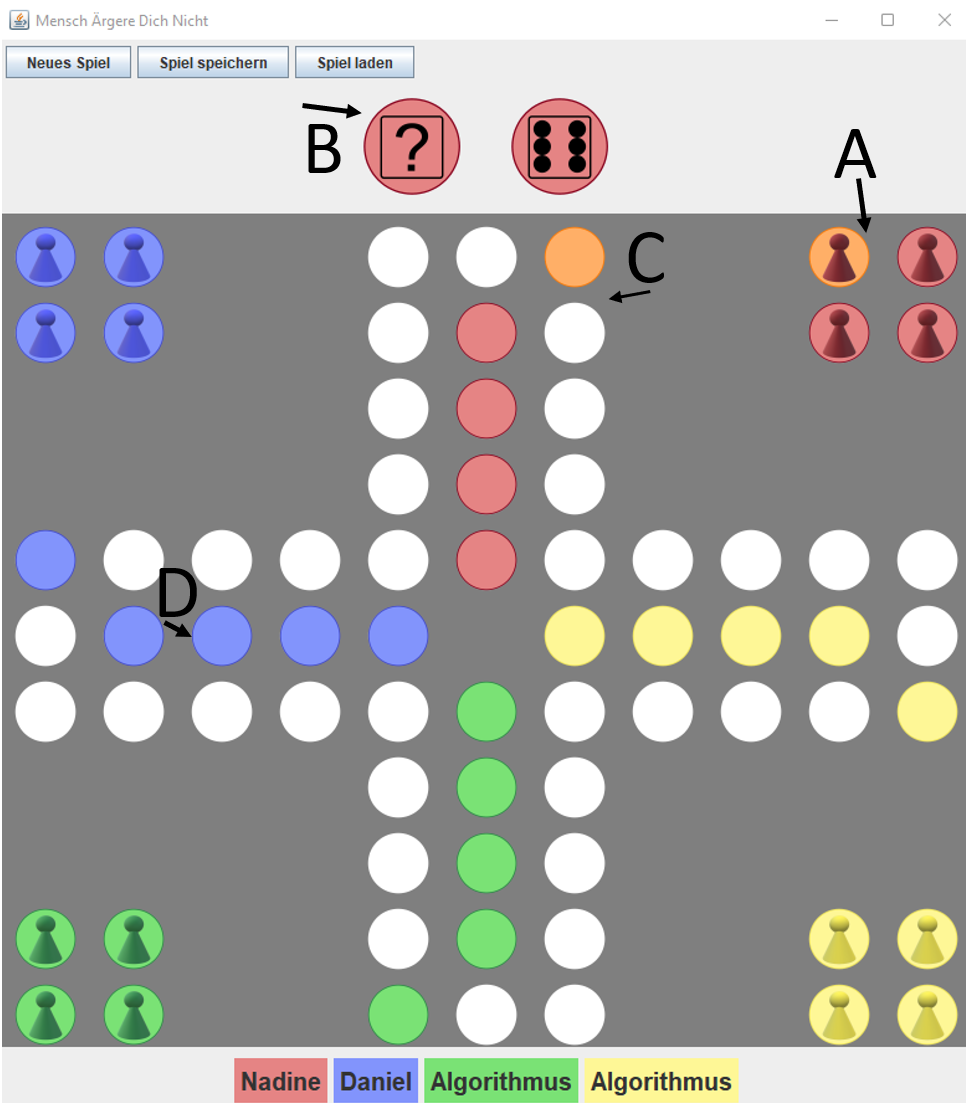
\includegraphics[scale=.6]{anleitung5}}
\caption{Hauptfenster der Anwendung mit Spielbrett}
\label{fig:anleitung5}
\end{figure}

% \newpage
% \titlespacing*{\chapter}{0pt}{-30mm}{10pt}
% \titleformat{\chapter}[display]
%   {\normalfont\bfseries}{}{10pt}{\Huge\thechapter.\quad}
  
% \chapter{Fragen an M. Müller}
% \pagestyle{scrheadings}
% \clearscrheadfoot
% \pagenumbering{arabic}
% \setcounter{page}{9}
% \ofoot[\pagemark]{\pagemark}
% %\ohead[\headmark]{\headmark}
% \onehalfspacing

% Fragen: 

% \begin{itemize}
%     %\item Dürfen wir \enquote{wir} in diesem Dokument verwenden?
%     %\item Wie genau soll die eigene Erklärung der Clean Architecture sein?
%     \item Siehe Kapitel SOLID / SRP: Ist es ok, dass wir die Klasse ControlMechanismFour nach refactoring nicht mehr haben?
%     \item Kapitel 3.2 OCP: Formulierung \enquote{Problem}
%     \item Kapitel 4.1 GRASP: Meint er mit negativ Beispiel einer geringen Kopplung eine starke Kopplung? 
%     \item Und soll die Kopplung in beiden fällen komplett aufgelöst werden oder nur zu einer geringen Kopplung gemacht werden?
%     \item Verstehen wir das richtig, dass man im DDD nur ein Repository haben kann, wenn man einen persistenten Speicher hat?
% \end{itemize}
%\include{kapitel6}
%\include{kapitel7}
\renewcommand{\bibname}{}
\clearscrheadfoot
\pagenumbering{Roman}
\setcounter{page}{9}
\ofoot[\pagemark]{\pagemark}
\vspace*{2.4cm}
\huge\textbf{Literaturverzeichnis}
\phantomsection
\addcontentsline{toc}{chapter}{Literaturverzeichnis}
\vspace*{.7cm}
\printbibliography[heading=none]

% Ab hier beginnt der Anhang
%\appendix
%\addcontentsline{toc}{chapter}{Anhang}
%
%\addcontentsline{toc}{chapter}{Index}
%\printindex
%
%\addcontentsline{toc}{chapter}{Literaturverzeichnis}

% Hat man das "biblatex"-Paket nicht installiert, benutzt man folgendes:
% Ohne das "biblatex"-Paket (s. bericht.sty) produziert folgendes
% "deutsche" Zitate in Literaturverzeichnissen gemaß der Norm DIN 1505,
% Teil 2 vom Jan. 1984.
% Die Zitatmarken werden alphabetisch nach Verfassern
% sortiert und sind durch abgekürzte Verfasserbuchstaben plus
% Erscheinungsjahr in eckigen Klammern gekennzeichnet.

% \bibliographystyle{alphadin}
% \bibliography{bericht}

%%%%%%%%%%%%%%%%%%%%%%%%%%%%%%%%%%%%%%%5
% BIBLATEX
% Benutzt man das "biblatex"-Paket, muss man folgendes schreiben:

%%%%%%%%%%%%%%%%%%%%%%%%%%%%%%%%%%%%%%%5


%\include{changelog}

%\newpage
%\addcontentsline{toc}{chapter}{Liste der ToDo's}
%\listoftodos[Liste der ToDo's]


\end{document}
